\documentclass[11pt,a4paper]{article}
\usepackage[T1]{fontenc}
\usepackage[utf8]{inputenc}
\usepackage{lmodern}
\usepackage{amsmath}
\usepackage[margin=2.3cm]{geometry}
\usepackage{microtype}
\usepackage{booktabs}
\usepackage{longtable}
\usepackage{tabularx}
\usepackage{array}
\usepackage{xcolor}
\usepackage{enumitem}
\usepackage{listings}
\usepackage{tikz}
\usetikzlibrary{arrows.meta,positioning,shapes.geometric,fit,calc}
\usepackage[hidelinks]{hyperref}

\setlist{itemsep=1pt,topsep=3pt}
\setlength{\parskip}{3pt}
\newcolumntype{L}{>{\raggedright\arraybackslash}X}
\newcommand{\code}[1]{\texttt{\hyphenchar\font=`\-\relax #1}}
\setlength{\emergencystretch}{3em}
\NewCommandCopy\origunderscore\_
\DeclareRobustCommand{\_}{\origunderscore\allowbreak}
\lstset{basicstyle=\ttfamily\small,columns=fixed,basewidth=0.52em,breaklines=true,frame=single,
  framesep=4pt,rulecolor=\color{black!30},xleftmargin=6pt,xrightmargin=6pt,
  literate={→}{{$\rightarrow$}}1 {≤}{{$\le$}}1 {≥}{{$\ge$}}1 {±}{{$\pm$}}1 {…}{{\ldots}}1 {‖}{{$\Vert$}}1}

\title{IceBridge: an Authenticated Peer-to-Peer Service Mesh over UDP,\\
with Rendezvous on the BitTorrent DHT\\[4pt]
\large Technical White Paper and Implementer's Specification}
\author{Angel Leon --- FrostWire}
\date{November 2026}

\begin{document}
\maketitle

\begin{abstract}
\noindent IceBridge is the peer-to-peer network that FrostWire for desktop 7.1 and FrostWire for Android 3.2 use for distributed
torrent search, catalog browsing and torrent metadata transfer. It has two parts. The
BitTorrent Mainline DHT is the directory: nodes publish signed identity records and index
manifests as BEP~44 mutable items, and announce themselves on well-known BEP~5 topics.
IceBridge proper is a transport and service mesh: a reliable UDP protocol (``rUDP'') whose
sessions are bound to Ed25519 identities, a bounded multi-hop relay, and an application
envelope that carries any protocol identified by a 16-bit number. Distributed search is one
such protocol. A node answers searches only from the torrents it is actively sharing, and
every answer is signed by the node that holds the torrent. This paper describes the problem
IceBridge solves, the design, and the wire formats, constants and procedures of the Java
implementation shared by FrostWire 7.1.3 for desktop and FrostWire 3.2.3 for Android (IceBridge
software version 1.1.0, rUDP protocol version~2). It is written so that an independent implementation, such as the planned Rust
one, can interoperate. Where the code and earlier design documents disagree, this paper
follows the code and records the difference. One difference matters more than the others:
rUDP version~2 authenticates every packet but does not encrypt anything. Payloads,
including search keywords and results, travel in clear text.
\end{abstract}

\tableofcontents
\newpage

%=====================================================================
\section{Problem}
%=====================================================================

BitTorrent moves content without a central server. Finding content does not work that way.
A user who wants a torrent usually searches a web site that keeps a central index of
\code{.torrent} files or magnet links. These index sites are single points of failure:

\begin{itemize}
\item They go offline. Many large index sites have closed after legal action, domain
  seizures, or because the operator stopped paying for hosting. Their indexes vanish with them.
\item They are easy to block. An ISP or a national firewall can block a handful of domain
  names and cut off search for millions of users, while the DHT and the swarms keep working.
\item They go stale. A central index lists torrents that nobody seeds any more. Users
  download dead magnets and wait.
\item They are a trust bottleneck. Users have to trust the site's moderation, uploader
  badges and comments, and the site sees every query.
\end{itemize}

The Mainline DHT (BEP~5) already gives every BitTorrent client a decentralized way to find
peers for a known info-hash. It cannot answer ``which torrents match these keywords''. The
DHT stores small values keyed by hashes. It has no keyword search, and storing an inverted
index in it would overload the nodes that happen to be close to popular keywords.

IceBridge closes that gap. It builds on what BitTorrent clients already run: the DHT, the
peers' own libraries of shared torrents, and their identities. The DHT is the directory and
IceBridge is the transport. Keyword queries go directly to the peers that hold the content,
and answers come back signed by those peers.

The maintainer's long-term goal is a network that, once enough peers join, makes central
torrent index sites largely unnecessary. Search results are fresh by construction, because a
peer only answers with torrents that its BitTorrent session is actively sharing. In
FrostWire's words: \emph{seeding is publishing}.

%=====================================================================
\section{Design goals and non-goals}
%=====================================================================

\subsection{Goals}
\begin{enumerate}
\item \textbf{No required central server.} Any node can find others through the DHT and
  the LAN. FrostWire's own servers make discovery faster but are optional (Section~\ref{sec:discovery}).
\item \textbf{Censorship resistance through decentralization.} No single domain or IP
  address needs to be reachable. Node endpoints are published on the DHT under topic hashes,
  and identities are self-certifying Ed25519 keys.
\item \textbf{Authenticated communication.} Every rUDP packet after the handshake is signed
  by its sender and bound to both endpoints and to the handshake transcript. Application
  messages such as search requests, search results, catalog pages and torrent metadata
  chunks carry their own end-to-end Ed25519 signatures. A relay cannot forge or alter them
  without detection.
\item \textbf{Protocol-agnostic transport.} IceBridge carries opaque payloads tagged with a
  16-bit protocol identifier (Section~\ref{sec:ibp1}). Search is protocol~1. Catalog browsing,
  metadata fetch, keyword digests and node metadata are other protocols. Chat, pub/sub, AI
  and file sync have reserved identifiers.
\item \textbf{Bounded resource use.} Every queue, cache, rate limiter, fan-out, hop count,
  fragment group and payload has a hard cap. Appendix~\ref{app:constants} lists them.
\item \textbf{Fresh results.} Only torrents active in the node's BitTorrent session are
  served (Section~\ref{sec:seeding}).
\item \textbf{Consent for bulk listing.} Answering keyword searches is part of joining the
  network. Listing a node's whole catalog to browsers and crawlers is a separate setting.
\end{enumerate}

\subsection{Non-goals}
\begin{enumerate}
\item \textbf{Content transfer.} IceBridge never carries torrent payload data. Downloads use
  ordinary BitTorrent. IceBridge carries only small control messages, search results, and
  \code{.torrent} metadata of at most 256~KiB.
\item \textbf{Anonymity.} A node's rUDP endpoint is public on the DHT. Peers it talks to
  see its IP address. IceBridge is not Tor or I2P.
\item \textbf{Confidentiality (in version 2).} The current protocol does not encrypt.
  Identities carry an X25519 public key and the code reserves key-derivation labels, but no
  encryption is implemented (Sections~\ref{sec:crypto-status} and~\ref{sec:future}).
\item \textbf{A global search index.} No node holds a complete index. Search reaches the
  peers that a bounded fan-out and keyword digests select.
\end{enumerate}

%=====================================================================
\section{Architecture overview}
%=====================================================================

\begin{figure}[ht]
\centering
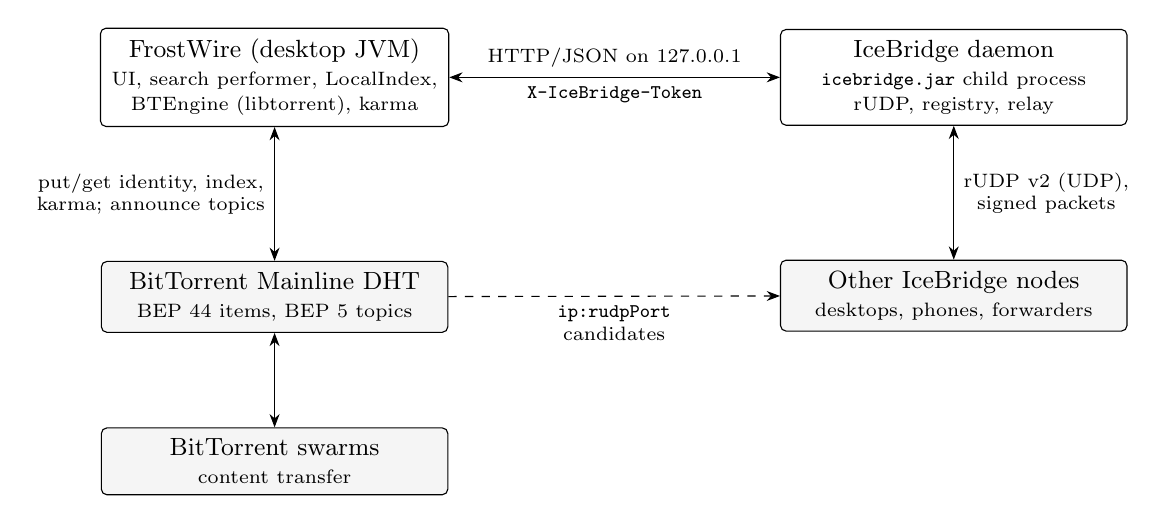
\begin{tikzpicture}[
  box/.style={draw,rounded corners=2pt,align=center,minimum height=8mm,inner sep=4pt,font=\small},
  lbl/.style={font=\scriptsize,align=center},
  >=Stealth]
\node[box,minimum width=44mm] (fw) {FrostWire (desktop JVM)\\[-1pt]\scriptsize UI, search performer, LocalIndex,\\[-2pt]\scriptsize BTEngine (libtorrent), karma};
\node[box,minimum width=44mm,right=42mm of fw] (ib) {IceBridge daemon\\[-1pt]\scriptsize \code{icebridge.jar} child process\\[-2pt]\scriptsize rUDP, registry, relay};
\draw[<->] (fw) -- node[lbl,above]{HTTP/JSON on 127.0.0.1}node[lbl,below]{\code{X-IceBridge-Token}} (ib);
\node[box,below=17mm of fw,minimum width=44mm,fill=black!4] (dht) {BitTorrent Mainline DHT\\[-1pt]\scriptsize BEP 44 items, BEP 5 topics};
\node[box,below=17mm of ib,minimum width=44mm,fill=black!4] (mesh) {Other IceBridge nodes\\[-1pt]\scriptsize desktops, phones, forwarders};
\draw[<->] (fw) -- node[lbl,left]{put/get identity, index,\\karma; announce topics} (dht);
\draw[<->] (ib) -- node[lbl,right]{rUDP v2 (UDP),\\signed packets} (mesh);
\draw[->,dashed] (dht) -- node[lbl,below]{\code{ip:rudpPort}\\candidates} (mesh);
\node[box,below=12mm of dht,minimum width=44mm,fill=black!4] (swarm) {BitTorrent swarms\\[-1pt]\scriptsize content transfer};
\draw[<->] (dht) -- (swarm);
\end{tikzpicture}
\caption{Processes and planes on a FrostWire desktop. On Android (3.2.x) the IceBridge server
runs inside the app process, and the app uses the same loopback control API. A standalone forwarder runs the daemon alone, with its own DHT session.}
\label{fig:arch}
\end{figure}

\subsection{Planes}
IceBridge has four planes.
\begin{description}
\item[Directory plane (DHT).] Signed identity records, catalog index manifests and karma
  chains are BEP~44 mutable items keyed by the node's Ed25519 public key. Endpoints are
  announced on four BEP~5 topics. See Section~\ref{sec:discovery}.
\item[Transport plane (rUDP).] One UDP socket per node, default port 6889 for servers and
  an automatically chosen port for desktops. Authenticated sessions, reliability,
  fragmentation, path migration and relaying. See Section~\ref{sec:transport}.
\item[Control plane.] A loopback HTTP/1.1 API through which the application registers
  identities, sends payloads, polls received payloads and asks the daemon to probe
  endpoints. See Section~\ref{sec:control}.
\item[Application plane.] Protocols carried in the IBP1 envelope: search, catalog, metadata,
  digests and node metadata. See Sections~\ref{sec:mesh} and~\ref{sec:services}.
\end{description}

\subsection{Deployments}
\begin{itemize}
\item \textbf{Desktop.} FrostWire launches \code{icebridge.jar} as a child JVM with
  \code{-{}-no-dht}. The parent process owns the DHT through its BitTorrent session, owns
  the local index, and answers searches. The child owns the UDP socket and the mesh.
\item \textbf{Android.} FrostWire for Android implements IceBridge since version 3.2.0
  (September 2026); the current release is 3.2.3. Phones and tablets are full IceBridge nodes
  that speak the same wire protocol as desktops and forwarders, so they search, answer
  searches, relay, and browse catalogs across the same mesh. The IceBridge server runs inside
  the app process rather than as a child JVM, with an automatically chosen rUDP port, a
  registry of up to 500 peers and a 180~s peer TTL. The app still talks to it through the same
  control API on an automatically chosen loopback port. The node's role defaults to
  \code{BOTH}; users can choose \code{CLIENT}, and the role profile of
  Table~\ref{tab:topology} is applied. The app's own BitTorrent session publishes the identity
  record and index manifest and announces on the DHT. On Wi-Fi the app holds Android's multicast
  lock while IceBridge runs, so that it can send and receive LAN beacons. Discovery and
  announces run every 300~s. A phone can instead use a \emph{remote} IceBridge
  node (an HTTPS URL and token), in which case it runs no node of its own and announces
  nothing.
\item \textbf{Standalone forwarder.} \code{icebridge.jar} runs alone, for example on a
  cloud host such as \code{virginia1.frostwire.com}. It starts a minimal libtorrent session
  with only the DHT enabled, so that it can announce itself and be found without any
  FrostWire GUI.
\end{itemize}

\subsection{Roles and capabilities}
A node has one of three roles: \code{FORWARDER} accepts inbound sessions and forwards
traffic; \code{CLIENT} only initiates; \code{BOTH} does both. In this paper an
\emph{ultrapeer} is a node with role \code{FORWARDER} or \code{BOTH}. Roles map to a 64-bit
capability mask (Table~\ref{tab:caps}) that identity records and \code{NODE\_META}
messages advertise.

\begin{table}[ht]
\centering\small
\begin{tabular}{rrll}
\toprule
Bit & Value & Name & Meaning\\
\midrule
0 & 1 & \code{RELAY} & forwards mesh traffic for others\\
1 & 2 & \code{SEARCH} & answers distributed search\\
2 & 4 & \code{INDEX} & keeps a local shared-torrent index\\
3 & 8 & \code{STORE} & reserved (storage)\\
4 & 16 & \code{DHT} & participates in the DHT\\
5 & 32 & \code{TORRENT} & runs a BitTorrent session\\
6 & 64 & \code{AI} & reserved\\
7 & 128 & \code{PUBLIC\_CATALOG} & answers catalog listing requests\\
\midrule
\multicolumn{4}{l}{Presets: \code{FORWARDER} = 17 (0x11), \code{CLIENT} = 54 (0x36), \code{BOTH} = 55 (0x37).}\\
\multicolumn{4}{l}{\code{fromRole} upper-cases with \code{Locale.ROOT}; unknown or null roles map to 55.}\\
\bottomrule
\end{tabular}
\caption{Capability bits (\code{NodeCapabilities}).}
\label{tab:caps}
\end{table}

%=====================================================================
\section{Identity}
\label{sec:identity}
%=====================================================================

\subsection{Keys}
Every node has a long-lived identity:
\begin{itemize}
\item An \textbf{Ed25519} key pair (RFC~8032). The 32-byte public key \emph{is} the node's
  identity everywhere in IceBridge: rUDP sessions, routing, DHT item keys, and signatures on
  search results, catalog pages, metadata and karma.
  The key pair is derived from a 32-byte seed exactly as RFC~8032 specifies (libtorrent's
  \code{ed25519\_create\_keypair}: SHA-512 of the seed, clamped), so standard libraries such
  as \code{ed25519-dalek} produce the same public key from the same seed.
\item An \textbf{X25519} key pair (RFC~7748). It is generated randomly and independently of
  the Ed25519 seed, published in the identity record, and \emph{not used} by any protocol
  today. It is reserved for future encryption.
\item A \textbf{node ID} of 20 bytes, defined as \code{SHA-1(ed25519\_pub)}. It is
  published but never checked by receivers, and it is unrelated to the node's libtorrent
  DHT node ID.
\end{itemize}

\paragraph{Proof of work.} When FrostWire creates a new identity it draws random seeds until
\code{SHA-1(ed25519\_pub)} has at least 20 leading zero bits, counted from the most
significant bit of byte~0 (\code{KarmaConstants.IDENTITY\_DIFFICULTY = 20}). This costs about
$2^{20}$ key generations. The check is \emph{not} enforced on remote peers, on imported
identities, or on identities restored from a seed phrase. Today it is informational, shown in
the Identity settings as ``identity difficulty''.

\paragraph{Seed phrase.} The 32-byte Ed25519 seed is shown to the user as a 24-word BIP39
English mnemonic. The seed itself is the BIP39 entropy: 256 bits plus an 8-bit SHA-256
checksum. No PBKDF2 stretching, passphrase or derivation path is applied. Input is
normalized with NFKC, lower-cased with \code{Locale.ROOT}, and split on runs of commas,
semicolons and white space. Exactly 24 words are required and the checksum is checked.
Restoring from the phrase recreates the Ed25519 key and generates a \emph{new} X25519 key.

\paragraph{Storage.} The identity lives in \code{<settings>/libtorrent/identity.dat}. The file
is four records, each a 4-byte big-endian length followed by DER bytes: Ed25519 PKCS\#8
private key, Ed25519 X.509 public key, X25519 PKCS\#8 private key, X25519 X.509 public key.
There is no magic number, version or encryption. The Ed25519 seed is at bytes 16--47 of the
PKCS\#8 record; the JDK prefix is \code{30 2e 02 01 00 30 05 06 03 2b 65 70 04 22 04 20}.
Importing or restoring an identity keeps one backup, \code{identity.dat.bak}. There is no
signed key rotation or revocation.

\paragraph{Raw key wrapping.} Java verifies raw 32-byte Ed25519 keys by prefixing the X.509
SubjectPublicKeyInfo header \code{30 2a 30 05 06 03 2b 65 70 03 21 00}. Implementations with
raw-key APIs do not need this.

\subsection{Identity record}
\label{sec:identity-record}
A node describes itself in a signed \emph{identity record}. The record is a bencoded
dictionary. Its canonical form follows BEP~3 bencoding with these extra rules, which the Java
decoder (\code{util/Bencode}) enforces on every signed structure:
keys sorted by their raw bytes, unique; integers in shortest form, no \code{-0}, no
\code{Long.MIN\_VALUE}; no trailing bytes; nesting depth at most 32; strings at most 1~MiB;
at most 65{,}536 items.

\begin{table}[ht]
\centering\small
\begin{tabularx}{\textwidth}{llcL}
\toprule
Key & Type & Since & Value\\
\midrule
\code{caps} & int & v3 & capability mask, Table~\ref{tab:caps}\\
\code{ed25519\_pub} & str & v1 & standard Base64 of the 32-byte key, no padding (43 chars)\\
\code{first\_seen} & int & v1 & Unix seconds, $>0$\\
\code{ib\_ver} & str & v4 & IceBridge software version, \code{"1.1.0"}\\
\code{last\_seen} & int & v1 & Unix seconds, $\ge$ \code{first\_seen}\\
\code{node\_id} & str & v1 & lowercase hex of the 20-byte node ID (40 chars)\\
\code{role} & str & v2 & \code{CLIENT}, \code{FORWARDER} or \code{BOTH}\\
\code{rudp\_port} & int & v2 & rUDP port\\
\code{sig} & str & v1 & standard Base64 of the 64-byte signature, no padding (86 chars)\\
\code{utp\_port} & int & v1 & legacy port; set to the rUDP port by current writers\\
\code{v} & int & v1 & record version, 1--4; writers emit 4\\
\code{x25519\_pub} & str & v1 & standard Base64 of the X25519 key, no padding\\
\bottomrule
\end{tabularx}
\caption{Identity record fields. Keys are shown in canonical (sorted) order.}
\label{tab:identity}
\end{table}

\paragraph{Signature.} The signature is pure Ed25519 (no pre-hash, no context) by the
identity key over the canonical bencoding of the dictionary \emph{without} the \code{sig} key
and containing only the keys defined for the record's version \code{v}.
A verifier must:
\begin{enumerate}
\item decode the dictionary and reject non-canonical bencoding;
\item check \code{1 <= v <= 4}, before narrowing it to a 32-bit integer;
\item read the fields for that version: v1 has no \code{rudp\_port}, \code{role},
  \code{caps} or \code{ib\_ver}; missing optional fields default to role \code{BOTH}, port~0,
  caps from the role, and version \code{""};
\item check lengths: node ID 20, keys 32, signature 64; \code{first\_seen > 0};
  \code{last\_seen >= first\_seen};
\item \emph{re-encode} the parsed fields in canonical form and verify the signature over
  those bytes with the embedded \code{ed25519\_pub};
\item when the record came from the DHT, check that \code{ed25519\_pub} equals the DHT item key.
\end{enumerate}
Because the signature covers re-encoded fields rather than the received bytes, unknown keys
are ignored and unsigned. A new field therefore needs a new version number. Upper-case hex,
padded Base64 or URL-safe Base64 in a record make verification fail.

The record has no expiry. Receivers do not check the node ID, the proof of work, the role
string or the capability mask. The publisher re-signs the record on every publication with
\code{first\_seen = last\_seen = now}.

%=====================================================================
\section{Transport: rUDP version 2}
\label{sec:transport}
%=====================================================================

rUDP is a small reliable-datagram protocol over one UDP socket. It gives each pair of nodes
an \emph{association} (session) that is bound to both Ed25519 identities. It provides
in-order reliable delivery, fragmentation of payloads up to 256~KiB, NAT rebinding, and a
relay frame for multi-hop delivery. Version~2 replaced the unauthenticated version~1. There
is no downgrade: version~1 packets are dropped.

\subsection{Packet header}
All integers are big-endian (network order). The header is 22 bytes.

\begin{table}[ht]
\centering\small
\begin{tabular}{rrll}
\toprule
Offset & Size & Field & Value\\
\midrule
0 & 2 & magic & \code{0x46 0x77} (``Fw'')\\
2 & 1 & version & 2\\
3 & 1 & type & Table~\ref{tab:rudp-types}\\
4 & 8 & connection ID (CID) & signed 64-bit, chosen by the initiator\\
12 & 4 & sequence & unsigned 32-bit semantics\\
16 & 4 & ack-through & highest in-order sequence received from the peer\\
20 & 2 & payload length & unsigned 16-bit; at most 1152\\
22 & $n$ & payload & exactly payload-length bytes\\
\bottomrule
\end{tabular}
\caption{rUDP packet header (\code{RudpPacket}, \code{RudpPacketCodec}).}
\label{tab:rudp-header}
\end{table}

A receiver silently drops a datagram that is shorter than 22 bytes, has the wrong magic or
version, has an unknown type, declares a payload longer than 1152 bytes
(\code{MAX\_WIRE\_PAYLOAD} = 1024 + 128), or whose length does not exactly match the remaining
bytes.

\begin{table}[ht]
\centering\small
\begin{tabularx}{\textwidth}{rlcL}
\toprule
Code & Type & Signed by & Use\\
\midrule
0x01 & \code{HELLO} & body sig & initiator opens a handshake\\
0x02 & \code{HELLO\_ACK} & body sig & responder answers\\
0x03 & \code{DATA} & packet & one application payload of at most 1024 bytes\\
0x04 & \code{DATA\_ACK} & packet & cumulative acknowledgement; empty body, sequence 0\\
0x05 & \code{HOLE\_PUNCH} & --- & \textbf{disabled in v2}: dropped on receipt, never sent\\
0x06 & \code{HOLE\_PUNCH\_RESPONSE} & --- & \textbf{disabled in v2}: dropped on receipt, never sent\\
0x07 & \code{RELAY} & packet & relay frame (Section~\ref{sec:relayframe})\\
0x08 & \code{RELAY\_RESPONSE} & packet & last hop of a relayed delivery\\
0x09 & \code{DATA\_FRAG} & packet & fragment of a larger payload\\
0x0A & \code{DATA\_END} & packet & last fragment\\
0x0B & \code{HELLO\_FINISH} & packet & initiator confirms the handshake\\
0x0C & \code{HELLO\_READY} & packet & responder confirms the handshake\\
0x0D & \code{PATH\_CHALLENGE} & packet & 32 random bytes to a new address\\
0x0E & \code{PATH\_RESPONSE} & packet & echo of the challenge\\
\bottomrule
\end{tabularx}
\caption{rUDP packet types. ``Packet'' means the packet is protected as described in
Section~\ref{sec:protect}.}
\label{tab:rudp-types}
\end{table}

\subsection{Handshake}
\label{sec:handshake}

\begin{figure}[ht]
\centering
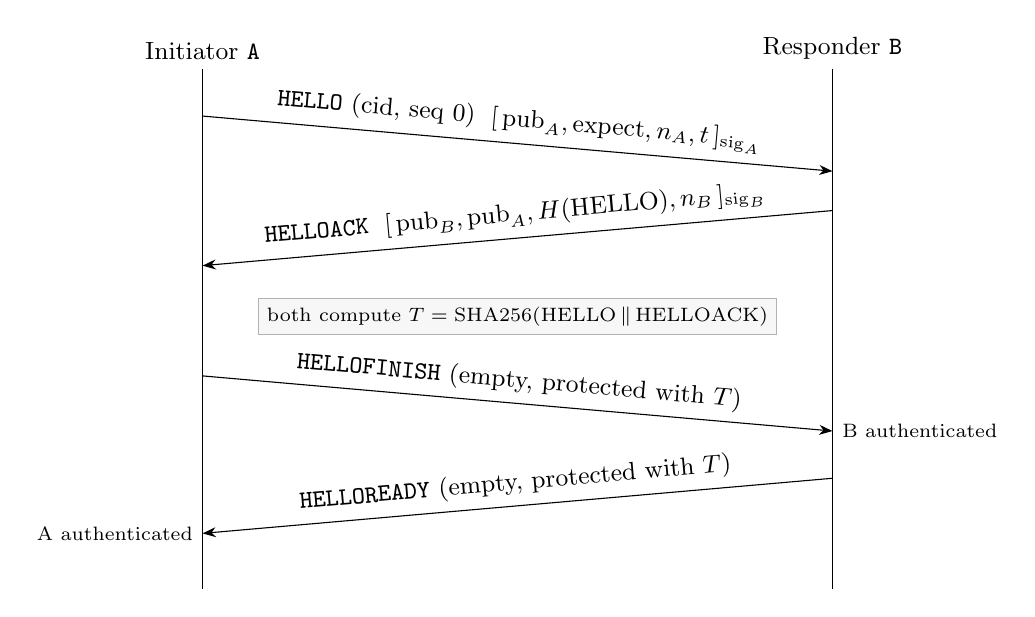
\begin{tikzpicture}[>=Stealth,font=\small]
\draw (0,0) node[above]{Initiator \code{A}} -- (0,-6.6);
\draw (8,0) node[above]{Responder \code{B}} -- (8,-6.6);
\draw[->] (0,-0.6) -- node[above,sloped]{\code{HELLO} (cid, seq 0) \;$[\,\mathrm{pub}_A, \mathrm{expect}, n_A, t\,]_{\mathrm{sig}_A}$} (8,-1.3);
\draw[->] (8,-1.8) -- node[above,sloped]{\code{HELLO\_ACK} \;$[\,\mathrm{pub}_B, \mathrm{pub}_A, H(\mathrm{HELLO}), n_B\,]_{\mathrm{sig}_B}$} (0,-2.5);
\node[draw=black!30,fill=black!3,font=\scriptsize,inner sep=3pt] at (4,-3.15) {both compute $T = \mathrm{SHA256}(\mathrm{HELLO} \,\Vert\, \mathrm{HELLO\_ACK})$};
\draw[->] (0,-3.9) -- node[above,sloped]{\code{HELLO\_FINISH} (empty, protected with $T$)} (8,-4.6);
\node[right,font=\scriptsize] at (8,-4.6) {B authenticated};
\draw[->] (8,-5.2) -- node[above,sloped]{\code{HELLO\_READY} (empty, protected with $T$)} (0,-5.9);
\node[left,font=\scriptsize] at (0,-5.9) {A authenticated};
\end{tikzpicture}
\caption{rUDP v2 handshake. ``Protected'' means signed as in Section~\ref{sec:protect}.}
\label{fig:handshake}
\end{figure}

The initiator picks a random CID that is not 0, not $-1$, and not already in use. Both sides
use the same CID for the association. Handshake packets have sequence 0 and ack-through 0.

\paragraph{Handshake signature input.} \code{HELLO} and \code{HELLO\_ACK} carry a body
followed by a 64-byte Ed25519 signature over:
\begin{lstlisting}
"FrostWire-IceBridge-rUDP-v2"   27 bytes, US-ASCII
u8   version (2)
u8   packet type (0x01 or 0x02)
i64  CID
body
\end{lstlisting}

\begin{table}[ht]
\centering\small
\begin{tabular}{rrl@{\qquad}rrl}
\toprule
\multicolumn{3}{c}{\code{HELLO} payload (168 bytes)} & \multicolumn{3}{c}{\code{HELLO\_ACK} payload (192 bytes)}\\
\cmidrule(r){1-3}\cmidrule(l){4-6}
Off & Len & Field & Off & Len & Field\\
\midrule
0 & 32 & initiator Ed25519 pub & 0 & 32 & responder Ed25519 pub\\
32 & 32 & intended responder pub, or zeros & 32 & 32 & initiator pub (HELLO[0..32])\\
64 & 32 & random challenge $n_A$ & 64 & 32 & SHA-256 of the full HELLO payload\\
96 & 8 & Unix time, seconds (i64) & 96 & 32 & random challenge $n_B$\\
104 & 64 & signature & 128 & 64 & signature\\
\bottomrule
\end{tabular}
\caption{Handshake payloads (\code{RudpAuth}).}
\label{tab:hello}
\end{table}

\paragraph{Responder rules.} The responder accepts a \code{HELLO} only if: the payload is
exactly 168 bytes; the timestamp is within $\pm 60$ seconds of its clock; the signature
verifies under the embedded initiator key; the intended-responder field is all zeros or equals
its own key; and the initiator is not itself. A zero intended-responder field is
\emph{identity discovery}: the initiator only knows an \code{ip:port} and learns the
responder's key from the answer. This proves that the endpoint holds the key. It does not
prove that the endpoint is a particular trusted node. If the same initiator retransmits an
identical \code{HELLO} from the same address, the responder resends its stored
\code{HELLO\_ACK}.

\paragraph{Initiator rules.} The initiator accepts a \code{HELLO\_ACK} only if it is exactly
192 bytes, bytes 32--63 equal its own key, bytes 64--95 equal SHA-256 of the \code{HELLO} it
sent, the responder key satisfies the intended-responder field, the signature verifies, and
the packet comes from the address it dialled.

\paragraph{Transcript and confirmation.} Both sides compute the transcript hash
\[ T = \mathrm{SHA256}(\text{HELLO payload} \,\Vert\, \text{HELLO\_ACK payload}) \]
over the complete payloads, signatures included. The initiator sends an empty protected
\code{HELLO\_FINISH}. The responder marks the association authenticated and answers with an
empty protected \code{HELLO\_READY}. The initiator then marks it authenticated. Data packets
(sequence $\ge 1$) are only sent after authentication. Both nodes record the peer's observed
address in their peer registry.

\paragraph{Simultaneous open.} If both nodes dial each other at once, each has an outbound
initiator session when the other's \code{HELLO} arrives. The node with the numerically
\emph{lower} public key (compared as unsigned bytes) ignores the inbound \code{HELLO} and
stays the initiator. The other node drops its own attempt, becomes the responder, and moves
its queued data into the new association. A fresh, valid \code{HELLO} from a peer that already
has an authenticated association, or whose earlier handshake stalled, replaces the old
association. This is how a restarted peer reconnects.

\subsection{Packet protection}
\label{sec:protect}
Every packet other than \code{HELLO} and \code{HELLO\_ACK} carries its body followed by a
64-byte Ed25519 signature by the sender's identity key over:
\begin{lstlisting}
"FrostWire-IceBridge-rUDP-v2"   27 bytes
u8   version (2)
u8   packet type
32   sender Ed25519 pub
32   recipient Ed25519 pub
32   transcript T
i64  CID
i32  sequence
i32  ack-through
i32  body length
body
\end{lstlisting}
The header's payload length is the body length plus 64. A receiver looks up the association
by CID. It rejects the packet if there is no association or transcript, if ack-through is
greater than the highest sequence it has sent, if the global packet rate limit is exhausted,
or if the signature does not verify. All of these checks happen before any session state or
routing changes. Addresses are deliberately not signed so that NAT rebinding works.

\subsection{Encryption status}
\label{sec:crypto-status}
rUDP version~2 provides \textbf{integrity and authentication, not confidentiality}. The
source code says so in \code{RudpAuth}: ``Ed25519 signatures provide integrity, NOT encryption
or forward secrecy.'' Concretely:
\begin{itemize}
\item No cipher is used anywhere in IceBridge: no AES, ChaCha20, or key agreement. The
  X25519 keys in identity records are generated and published but never used. The labels
  \code{frostwire-icebridge-session-v1}, \code{frostwire-relay-transport-v1} and
  \code{frostwire-search-v1} are defined and referenced by no code.
\item Every rUDP payload, every relay frame, and every application message travels in clear
  text. That includes search keywords, result rows, catalog pages and \code{.torrent} bytes.
  A network observer or a relay node can read them.
\item What the signatures do provide: a packet cannot be injected, altered, replayed into
  another association, or reflected between directions without detection. Application
  messages carry their own end-to-end signatures, so a relay cannot forge a search result,
  catalog page or metadata chunk.
\item There is no forward secrecy, because there are no session keys.
\item The control API is plain HTTP on the loopback interface, protected by a bearer token.
\end{itemize}

\subsection{Reliability}
Each association keeps one outgoing sequence counter starting at 1 and one ``received
through'' counter starting at 0. Sequence numbers are compared as unsigned 32-bit integers.
Sequence 0 is reserved for handshake, acknowledgement and path packets. When the counter
would wrap past $2^{32}-1$ to 0, the association must be re-established.

\begin{itemize}
\item \textbf{In-order only.} A receiver accepts a sequenced packet only if it is exactly
  received-through + 1. It drops later packets (gaps) without buffering them. For a duplicate
  or old packet it resends a \code{DATA\_ACK}. The protocol is effectively go-back-N.
\item \textbf{Acknowledgement.} After the application accepts a packet, the receiver
  advances its counter and sends \code{DATA\_ACK} (sequence 0, empty body, ack-through =
  received-through). Data packets also carry ack-through. An ACK means the next hop has taken
  ownership of the payload under its bounded queues. It does not mean the remote application
  processed it.
\item \textbf{Backpressure.} If the application queue refuses a payload, the packet is not
  acknowledged, and the sender retransmits it later.
\item \textbf{Window.} At most 32 unacknowledged sequenced packets are in flight per
  association (\code{SEND\_WINDOW}).
\item \textbf{Retransmission.} A timer runs every 500~ms. A packet is resent when
  $500 \cdot 2^{\min(r,3)}$~ms have passed since it was last sent, where $r$ is its retry
  count. The schedule is 500, 1000, 2000, 4000, 4000~ms. If any pending packet reaches 5
  retries, or 15~s since it was first sent, the \emph{whole association} is dropped. The
  application must retry at its own level.
\item \textbf{Idle timeout.} An authenticated association is dropped after 120~s without
  activity; an unauthenticated one after 15~s.
\end{itemize}

\subsection{Fragmentation}
A payload larger than 1024 bytes (\code{MAX\_FRAGMENT\_PAYLOAD}) is split into
$k = \lceil n / 1024 \rceil$ fragments. Each fragment is a sequenced packet whose body is:
\begin{center}\small
\begin{tabular}{rrl}
\toprule
Offset & Size & Field\\
\midrule
0 & 4 & group ID (random i32, per payload)\\
4 & 4 & fragment index, 0-based\\
8 & 4 & fragment total $k$\\
12 & $\le$1024 & fragment data\\
\bottomrule
\end{tabular}
\end{center}
Fragments $0..k-2$ have type \code{DATA\_FRAG} and the last has type \code{DATA\_END}.
The receiver requires fragments in index order and allows no other data type while a group is
open. Limits: $k \le 256$; assembled size at most 256~KiB (262{,}144 bytes); at most 64
groups pending per node; a group older than 30~s ends the association. With the 12-byte
header and the 64-byte signature, the largest protected payload is 1100 bytes, and the largest
datagram is 1122 bytes, well under a 1500-byte MTU.

\subsection{Path migration}
When an authenticated packet with a valid signature arrives from a new address (for example
after a NAT rebinding on a phone), the receiver does not process it. Instead it sends a
protected \code{PATH\_CHALLENGE} with 32 random bytes to the new address. If a protected
\code{PATH\_RESPONSE} with the same bytes comes back from that address within 5~s, the
association moves to the new address. At most one challenge is outstanding per association
every 5~s. A replayed packet therefore can never move an association by itself.

\subsection{Admission control}
Checks are ordered so that cheap checks come before signature verification:
\begin{itemize}
\item \code{HELLO}/\code{HELLO\_ACK}: a global token bucket (burst 200, 50/s) and then a
  per-source-IP bucket (burst 10, 2/s, at most 4096 IP buckets). Outbound dials share the
  global bucket.
\item Other packets: a global bucket of 2000/s (burst 2000) before signature verification.
\item Associations: at most $\min(\text{maxSessions}, 4096)$ in total, where
  \code{maxSessions} defaults to 1024. At most 256 per IPv4 /24 or IPv6 /64.
\item Retained data: per association 512 packets and 1~MiB; per node 16{,}384 packets and
  16~MiB. Received datagrams pass through one FIFO worker with a 4096-entry queue. When the
  queue is full, the newest datagram is dropped and rUDP retransmission recovers it.
\end{itemize}

\subsection{NAT traversal}
Version~2 has \emph{no hole-punching protocol}. The \code{HOLE\_PUNCH} types exist but are
dropped on receipt, because there is no authenticated way yet for a target to consent to an
introduction. Earlier changelog entries (7.1.0) describe \code{HOLE\_PUNCH} as implemented.
That is no longer true. Nodes behind NAT are reached in three ways:
\begin{enumerate}
\item The NAT-ed node dials out to ultrapeers. The resulting association keeps the NAT
  mapping open. Leaves ping their uplinks at least every 30~s through \code{PeerRegistrySync},
  which is shorter than the 120~s idle timeout.
\item Messages for a NAT-ed node go through a relay that already has an association with it
  (Section~\ref{sec:relayframe}).
\item Two NAT-ed nodes that dial each other at the same moment may connect through the
  simultaneous-open rule. Nothing coordinates such an attempt.
\end{enumerate}
On a LAN, nodes find each other's private addresses through multicast
(Section~\ref{sec:lan}), because most routers do not support hairpin connections to their own
public address.

\subsection{Relay frame}
\label{sec:relayframe}
A \code{RELAY} packet body is a relay frame:
\begin{center}\small
\begin{tabular}{rrl}
\toprule
Offset & Size & Field\\
\midrule
0 & 32 & source pub: the \emph{sending hop's} key\\
32 & 32 & target pub: the final recipient's key\\
64 & 1 & hop TTL (u8)\\
65 & 1..959 & application payload (\code{MAX\_APP\_PAYLOAD} = 1024 $-$ 65)\\
\bottomrule
\end{tabular}
\end{center}
Relay frames are never fragmented, so a relayed payload is at most 959 bytes including the
6-byte IBP1 envelope. Delivery works as follows (\code{RudpSessionManager.deliver},
\code{handleRelay}, \code{forward}):
\begin{enumerate}
\item The sender delivers directly when it can: to itself, to a co-located client through the
  local poll queue, over a live association, or by dialling the target's registered address.
\item If that fails and the payload is at most 959 bytes, the sender \emph{floods}: it sends
  a \code{RELAY} frame with TTL = \code{meshHopTtl} (3) to up to \code{meshBroadcastFanout}
  forwarders from its registry. The forwarders are shuffled, with at most 2 per IPv4 /24.
\item A forwarder accepts a frame only if its source pub equals the authenticated key of the
  association it arrived on, and its TTL is at most 6.
\item If the target is the forwarder itself, it delivers locally. If the target is in its
  registry, it sends a \code{RELAY\_RESPONSE} to the target, with body
  \code{source pub (32) || payload}, over an existing or newly dialled association.
\item Otherwise, if TTL $> 0$, it forwards a new frame with the TTL reduced by 1 to its own forwarders,
  excluding the hop it came from. The new frame carries the forwarder's own key as source.
\end{enumerate}
The recipient's application sees the \emph{last hop's} key as the transport source of a
relayed message. The original sender's identity is carried and verified only inside the
signed application message. Flooding keeps no duplicate-suppression cache. TTL and the
exclusion of the previous hop bound it, and applications drop duplicates through their own
nonces and replay caches. The worst case is about $N + N^2 + N^3$ frames for fan-out $N$ and
TTL 3, so forwarders cap their fan-out (Table~\ref{tab:topology}).

%=====================================================================
\section{Discovery and the DHT}
\label{sec:discovery}
%=====================================================================

\subsection{Why the DHT and IceBridge fit together}
\label{sec:synergy}
The BitTorrent Mainline DHT has millions of nodes, has no owner, and every BitTorrent client
already runs it. It is good at two things: storing small signed values under a public key
(BEP~44), and remembering which \code{ip:port} pairs announced themselves under a 20-byte key
(BEP~5). It cannot carry conversations, answer keyword queries, or reach a node behind NAT.

IceBridge is good at exactly those things. It does not have its own directory and does not
need one. The split is:

\begin{center}\small
\begin{tabularx}{\textwidth}{lLL}
\toprule
 & BitTorrent DHT (directory) & IceBridge (transport and services)\\
\midrule
Stores & signed identity records, catalog manifests, karma chains (BEP~44) & nothing durable; peer registry and host cache in memory or on local disk\\
Finds & endpoints on the bootstrap, relay, peer and heartbeat topics (BEP~5) & the key behind an endpoint (rUDP handshake), then routes by key\\
Carries & at most 1000 bytes per item, no messages & reliable sessions, payloads up to 256~KiB, multi-hop relay\\
Trust & item signatures by the owner's key & the same key: sessions, messages and results are signed with it\\
Reach & public addresses only & NAT-ed nodes through outbound sessions and relays\\
\bottomrule
\end{tabularx}
\end{center}

The same Ed25519 key is the DHT item key, the rUDP session identity, and the signer of every
search result. A node that finds an endpoint on a DHT topic proves who is behind it with an
rUDP handshake, then looks up that key's signed identity record on the DHT to learn its role,
capabilities and version. A user who receives a signed result from a key can fetch that key's
catalog manifest and karma chain from the DHT, without contacting the node. Neither half
needs a server that FrostWire runs.

\subsection{BEP 44 mutable items}
FrostWire publishes three items per identity. The code and older documents call them
``BEP~46'' items. They are BEP~44 mutable items with a salt. No BEP~46 info-hash pointers are
used.

\begin{table}[ht]
\centering\small
\begin{tabularx}{\textwidth}{lllL}
\toprule
Item & Key & Salt (US-ASCII) & Value\\
\midrule
Identity & Ed25519 pub & \code{frostwire-identity-v1} & signed identity record, \code{sig} included (Table~\ref{tab:identity})\\
Index manifest & Ed25519 pub & \code{frostwire-index-v1} & catalog manifest (Section~\ref{sec:dht-index})\\
Karma chain & Ed25519 pub & \code{frostwire-karma-v1}, \code{frostwire-karma-v1/<n>} & karma head page, older pages (Section~\ref{sec:karma})\\
\bottomrule
\end{tabularx}
\caption{BEP 44 mutable items.}
\label{tab:bep44}
\end{table}

As BEP~44 specifies, the item target is $\mathrm{SHA1}(\mathrm{pub} \,\Vert\, \mathrm{salt})$,
and the item signature covers \code{4:salt<len>:<salt>3:seqi<seq>e1:v<bencoded value>}.
Puts go through libtorrent's \code{dht\_put\_item} with a callback. libtorrent first fetches
the current item, then the callback sets the value, increments the sequence number and
signs. The sequence number is therefore the highest one seen plus one, or 1 for a new item.
The application never chooses it. The 64-byte secret key passed to libtorrent is the expanded
Ed25519 key, SHA-512 of the seed after clamping, not \code{seed || pub}.

Gets use \code{dht\_get\_item} with a timeout in whole seconds (5~s for identity, index and
karma). The Java binding returns the \emph{first} matching item alert. libtorrent can post a
non-authoritative alert before the lookup finishes, so the result may not have the highest
sequence number. A new implementation should wait for the authoritative result.

Republish intervals: identity at most every 300~s; index manifest when it changes or every
300~s; karma pages every 1800~s and right after each endorsement.

\subsection{BEP 5 topics}
A topic's info-hash is $\mathrm{SHA1}$ of the topic's US-ASCII bytes.

\begin{table}[ht]
\centering\small
\begin{tabularx}{\textwidth}{lL}
\toprule
Topic string & Who announces\\
\midrule
\code{frostwire-bootstrap-v1} & dedicated servers started with \code{-{}-bootstrap} (default for \code{FORWARDER} via environment). Looked up first.\\
\code{frostwire-relays-v1} & role \code{FORWARDER} or \code{BOTH}; a \code{CLIENT} only if marked connectable (no code marks it today)\\
\code{frostwire-peers-v1} & every desktop, Android nodes with an embedded server, and standalone daemons whose role is not \code{FORWARDER}\\
\code{frostwire-heartbeat-v1-<h>} & every node; $h = \lfloor \mathrm{epochMillis} / 3\,600\,000 \rfloor$ in decimal (the hour number). Used by crawlers to count presence.\\
\bottomrule
\end{tabularx}
\caption{BEP 5 announce topics.}
\label{tab:topics}
\end{table}

Announces use \code{dht\_announce} with flags 0: no \code{implied\_port}, not a seed. The
announced port is the node's \emph{rUDP} port, or the legacy port if the rUDP port is
unknown. A node must not announce port~0. Desktop nodes announce every 30~s, Android every
300~s, standalone daemons every 60~s.

The desktop child process runs with \code{-{}-no-dht}, and the parent announces through its
BitTorrent session. A standalone daemon starts its own libtorrent session with only the DHT,
on an ephemeral UDP port separate from rUDP, using the routers
\code{dht.libtorrent.org:25401}, \code{router.bittorrent.com:6881},
\code{dht.transmissionbt.com:6881} and \code{router.silotis.us:6881}. If the DHT fails to
start, the daemon keeps running without it.

Lookups use \code{dht\_get\_peers}. The Java binding returns after the first reply alert,
that is, the first responding DHT node's peer list. A new implementation should collect
replies from all nodes.

\subsection{Discovery pass}
A discovery pass runs every 30~s on desktop and every 300~s on Android. It gathers candidate
\code{ip:rudpPort} endpoints from three sources, in order:
\begin{enumerate}
\item \textbf{Host cache and seeds} (preferred). The local host cache
  (Section~\ref{sec:hostcache}) and the built-in seed \code{virginia1.frostwire.com:6889}.
  The system property \code{frostwire.icebridge.seeds} replaces the seeds with a
  comma-separated list; an empty value disables them.
\item \textbf{LAN beacon} (preferred). Private IPv4 senders heard on the multicast group.
\item \textbf{DHT}, with a 5~s budget: \code{frostwire-bootstrap-v1} for up to 2~s (results
  preferred), then \code{frostwire-relays-v1} for up to 3~s, then \code{frostwire-peers-v1}
  for what remains. Deduplicated by \code{host:port}, at most 64 candidates.
\end{enumerate}
The pass drops loopback, link-local, multicast and own-interface addresses, our own public
address on our own rUDP port, and endpoints in back-off. It orders preferred candidates
first and shuffles the rest, takes at most 64, and probes them in parallel: 16 at a time,
3~s per probe, 15~s per pass.

A \textbf{probe} is an rUDP identity-discovery handshake (zero intended responder). The daemon
exposes it as \code{POST /probe} and the caller polls it every 100~ms. When the handshake
completes, the prober fetches the key's identity record from the DHT to learn its
capabilities and version, then registers the peer as verified. If our own key answers, that
endpoint is muted for 10~minutes. Failed endpoints back off from 30~s, doubling up to
10~minutes. Preferred endpoints back off from 5~s, doubling up to 60~s.

\subsection{Host cache}
\label{sec:hostcache}
The host cache is a UTF-8 text file at \code{\~{}/.frostwire/icebridge\_host\_cache.txt}
(on Android, under the app's \code{libtorrent} directory). It begins with a \code{\#}
comment line, and each further line is
\code{host:port,ROLE,lastSuccessfulPingMs,consecutiveFailures}. The port is the rUDP
port. The host is everything before the last colon, so IPv6 addresses are stored without
brackets. Ultrapeers that answer a probe are added. An entry is removed after 5 consecutive
failures. There is no size cap. Writes go to a temporary file that is then renamed, and
happen at most once every 5~minutes, plus at shutdown.

\subsection{LAN multicast beacon}
\label{sec:lan}
Every 10~s a node sends the ASCII text \code{"FWIB1 <rudpPort>"} to
\code{239.255.70.88:6890} on each active, multicast-capable, non-loopback,
non-point-to-point IPv4 interface. It listens on \code{0.0.0.0:6890} with
\code{SO\_REUSEADDR}. A receiver accepts a datagram only if: it is at most 64 bytes; it is
\code{FWIB1}, a space, and 1--5 digits forming a port from 1 to 65535; and the sender
is an RFC~1918 private IPv4 address. Candidates expire after 120~s, with at most 128 kept.
The beacon is not signed. It only produces candidates, and the rUDP handshake authenticates
them.

\subsection{DHT index manifest}
\label{sec:dht-index}
A node that shares its catalog (Section~\ref{sec:seeding}) publishes a manifest of its
public torrents under salt \code{frostwire-index-v1}:
\begin{lstlisting}
{ "pub": <std Base64 of pub, no padding>,
  "rows": [ {"fc": <file count>, "ih": <hex info-hash>, "n": <name>, "s": <size>}, ... ],
  "ts": <Unix seconds>, "v": 1 }                      (bencoded, keys sorted)
\end{lstlisting}
Rows are sorted by most recently seen. They are added while the bencoded manifest stays
within 950 bytes, so the manifest holds only the first few torrents. The full catalog is
available through mesh browsing (Section~\ref{sec:catalog}). The manifest has no signature
of its own. Only the BEP~44 item signature protects it. When the user stops sharing the
catalog, or nothing is public, an empty \code{rows} list replaces the previous manifest.

%=====================================================================
\section{Relay mesh, topology and control API}
\label{sec:mesh}
%=====================================================================

\subsection{The IBP1 application envelope}
\label{sec:ibp1}
Every payload the application hands to IceBridge is wrapped in a 6-byte envelope:
\begin{center}\small
\begin{tabular}{rrl}
\toprule
Offset & Size & Field\\
\midrule
0 & 4 & magic \code{"IBP1"} (\code{49 42 50 31})\\
4 & 2 & protocol ID, u16 big-endian\\
6 & $\ge 1$ & payload (to the end of the rUDP payload; no length field)\\
\bottomrule
\end{tabular}
\end{center}
When wrapping, protocol ID~0 is changed to 1. When unwrapping, the raw ID is returned. A
received ID~0 is treated as \code{SEARCH} by the application. Unknown IDs are delivered and
logged, never rejected. This makes the transport independent of content: a new service only
needs a new ID.

\begin{table}[ht]
\centering\small
\begin{tabularx}{\textwidth}{rlL}
\toprule
ID & Name & Use\\
\midrule
0 & \code{UNSPECIFIED} & treated as \code{SEARCH}\\
1 & \code{SEARCH} & distributed search request and response (Section~\ref{sec:search})\\
2 & \code{CHAT} & reserved\\
3 & \code{METADATA} & \code{TORRENT\_FETCH} request and chunks (Section~\ref{sec:fetch})\\
4 & \code{PUBSUB} & reserved\\
5 & \code{AI} & reserved\\
6 & \code{TELEMETRY} & ping: the single byte \code{0x01}\\
7 & \code{FILESYNC} & reserved\\
8 & \code{INDEX\_DIGEST} & keyword Bloom filter of a node's index\\
9 & \code{NODE\_META} & capability mask: \code{[0x01][caps i64 BE]}, exactly 9 bytes\\
10 & \code{CLUSTER\_DIGEST} & union of an ultrapeer's own and its leaves' digests\\
11 & \code{CATALOG} & catalog browse request and pages (Section~\ref{sec:catalog})\\
\bottomrule
\end{tabularx}
\caption{Mesh protocol IDs (\code{MeshProtocolId}).}
\label{tab:protoids}
\end{table}

\subsection{Topology}
IceBridge borrows the two-tier shape of Gnutella with ultrapeers. Ultrapeers keep
associations with many other ultrapeers and leaves. Leaves keep a few uplinks. The values
below are what runs: \code{IceBridgeConfig.fromEnv} applies a per-role profile on top of the
compiled defaults. Environment variables \code{ICEBRIDGE\_MESH\_FANOUT},
\code{ICEBRIDGE\_SEARCH\_PEER\_FANOUT}, \code{ICEBRIDGE\_MESH\_HOP\_TTL},
\code{ICEBRIDGE\_SEARCH\_TTL}, \code{ICEBRIDGE\_SOFT\_MAX} and
\code{ICEBRIDGE\_LEAF\_UP\_CONNECTIONS} override them.

\begin{table}[ht]
\centering\small
\begin{tabular}{lrrrr}
\toprule
Parameter & Compiled default & Ultrapeer profile & Leaf profile & Hard max\\
\midrule
mesh broadcast fan-out $N$ & 6 & 32 & 6 & 96\\
search peer fan-out $M$ & 8 & 32 & 6 & 96\\
mesh hop TTL & 3 & 3 & 3 & 6\\
search TTL & 2 & 7 & 7 & 7\\
soft max (hops + TTL) & 3 & 7 & 7 & 7\\
leaf uplinks & 3 & 6 & 6 & 16\\
\bottomrule
\end{tabular}
\caption{Topology parameters (\code{IceBridgeTopology}). The standalone daemon, the desktop
and Android apply the role profile; a server built in code that does not apply it keeps the
compiled defaults.}
\label{tab:topology}
\end{table}

\paragraph{Peer registry sync.} On a FrostWire node, \code{PeerRegistrySync} runs every
30~s and keeps the daemon's registry and the application's peer directory consistent:
\begin{enumerate}
\item it registers its own identity with the daemon (signed \code{/register});
\item it pushes up to 100 verified peers, ranked by trust, as routes;
\item it pulls up to 100 routes from \code{/lookup}, ignoring entries more than 10~minutes old;
\item it pings uplinks (\code{TELEMETRY} \code{0x01}): 32 ultrapeers if it is one, otherwise 6;
\item it sends its \code{INDEX\_DIGEST} to 6 ultrapeers when the digest changes, or at
  least every 120~s;
\item an ultrapeer sends a \code{CLUSTER\_DIGEST} to 32 ultrapeers at most every 120~s;
\item it sends \code{NODE\_META} to 16 ultrapeers at most every 120~s.
\end{enumerate}

\paragraph{Keyword digests.} An \code{INDEX\_DIGEST} payload is \code{0x01} followed by a
Bloom filter whose length is a power of two between 64 and 16{,}384 bytes (4096 for a leaf,
16{,}384 for a cluster), with $k = 4$ hash functions. For hash $i \in \{0..3\}$:
$h_i$ is the first 8 bytes, read big-endian, of $\mathrm{SHA256}(\mathrm{byte}(i) \,\Vert\,
\mathrm{UTF8}(\mathit{token}))$. The bit index is the top $\log_2(\mathit{bits})$ bits of
$h_i$, set as \code{byte[b>>3] |= 1 << (b \& 7)}. Tokens come from NFD normalization,
removal of combining marks, lower-casing with \code{Locale.ROOT}, and runs of ASCII
\code{[a-z0-9]} of length at least 3, minus stop words. At most 2048 tokens are taken from at
most 16{,}384 input characters. A query of $n$ tokens matches if at least $n$ tokens hit
when $n \le 2$, otherwise at least $\lfloor (2n+2)/3 \rfloor$. Digests let searchers and
forwarders choose likely holders first. A false positive costs one extra query, and a false
negative cannot happen for indexed tokens. Note that the tokenizer is ASCII-only, so names in
non-Latin scripts produce no tokens and gain nothing from digests.

\subsection{Control API}
\label{sec:control}
The application talks to its IceBridge daemon over HTTP/1.1 on \code{127.0.0.1}. The desktop
launches the child with \code{-{}-control-http-port 0}. The child prints a line
\code{ICEBRIDGE\_CONTROL\_PORT=<port>} on standard output, and the parent reads it. There is
no announcement file. Every endpoint except \code{/health} requires the header
\code{X-IceBridge-Token}. The parent generates the token as 32 random bytes in lowercase hex
and hands it over in an owner-only file (\code{-{}-auth-tokens-file}), never on the command
line. Tokens are compared in constant time. Request bodies are JSON and at most 64~KiB.
Responses are \code{\{"ok":true,"data":...\}} or \code{\{"ok":false,"error":"..."\}}. Binary
values are Base64url without padding. Unknown endpoints return HTTP 400; there is no 404.

\begin{longtable}{p{0.24\textwidth}p{0.70\textwidth}}
\toprule
Endpoint & Purpose\\
\midrule\endhead
\code{GET /health} & liveness; no token\\
\code{POST /register} & signed self-registration: \code{\{pub, host, rudpPort, role, timestamp, icebridgeVersion, signature\}}. The signature is Ed25519 over the UTF-8 bytes of \code{len(pub):pub|len(host):host|rudpPort|ROLE|timestamp} plus \code{|len(v):v} if a version is given, where \code{len} counts UTF-16 units and \code{pub} is the Base64url string. Timestamp within $\pm 60$~s.\\
\code{POST /route} & unsigned route hint \code{\{pub, host, rudpPort, role, ifAbsent\}}\\
\code{POST /consumer} & subscribe or unsubscribe a per-identity inbound queue\\
\code{POST /probe} & rUDP identity discovery of \code{\{host, port, cancel\}}; returns \code{none}, \code{pending} or \code{established} with \code{pub}\\
\code{GET /lookup} & up to 100 registry entries \code{\{pub, host, rudpPort, role, lastSeenMs, icebridgeVersion\}}\\
\code{POST /send} & \code{\{targetPub, payload, protocolId\}}: wrap in IBP1 and deliver\\
\code{GET /poll} & drain up to 256 messages (256~KiB) \code{\{sourcePub, payload, receivedMs, protocolId\}}; not long-polling; messages are removed when returned\\
\code{GET /metrics} & cumulative counters (packets, bytes, rejections, registry size)\\
\code{GET /events} & recent event log (ring buffer of 5000)\\
\code{GET /catalog} & browse a peer's catalog (timeout 100--30{,}000~ms, default 5000)\\
\code{GET /torrent} & \code{TORRENT\_FETCH} by info-hash from a holder (default 15{,}000~ms)\\
\bottomrule
\end{longtable}

Inbound queues hold at most 512 messages each, 256 consumers, 4096 messages and 16~MiB in
total. The desktop polls every 300~ms. The parent supervises the child: it checks
\code{/health} every 10~s, restarts the child on failure, and keeps the same rUDP port across
restarts. The child exits when the parent's PID disappears (checked every 3~s).

%=====================================================================
\section{Services}
\label{sec:services}
%=====================================================================

All service messages are UTF-8 JSON objects, produced by Gson. Method names in the code say
``bencode'', but the wire format is JSON. Binary fields use \emph{standard} Base64 without
padding, unless noted. Hex is written in lowercase and read in either case. Timestamps are
Unix seconds and must be within $\pm 300$~s of the receiver's clock. Signatures are pure
Ed25519 by the sender's identity key over a byte string built as described, not over the
JSON. In the signature layouts below, \code{i32}/\code{i64} are big-endian and
\code{lp(x)} means \code{i32 length || x}.

\subsection{Distributed search (protocol 1)}
\label{sec:search}

\paragraph{Request} (\code{RemoteSearchRequest}, version 3):
\begin{lstlisting}
{"v":3, "k":<keywords>, "lim":<1..100>, "nonce":<32 bytes>, "ttl":<int>, "maxTtl":<int>,
 "pub":<requester pub>, "path":[<pub>, ...], "ts":<seconds>, "sig":<64 bytes>}
\end{lstlisting}
Signed bytes:
\begin{lstlisting}
i32 v | lp(UTF-8 keywords) | i32 lim | lp(nonce) | lp(requester pub) | i64 ts | i32 maxTtl
\end{lstlisting}
\code{ttl} and \code{path} are not signed, so forwarders can change them within the signed
\code{maxTtl}. A receiver checks: all fields present; \code{v = 3}; keywords at most 1024 UTF-8
bytes; \code{0 < lim <= 100}; \code{path} has at most 8 unique 32-byte keys;
$0 \le \mathit{ttl}$, $\mathit{maxTtl} \le 8$, $|\mathit{path}| \le \mathit{maxTtl}$, and
$\mathit{ttl} \le \mathit{maxTtl} - |\mathit{path}|$. Keywords are sent as typed. Each
responder normalizes them for its own index.

\paragraph{Originating a search.} The searcher picks peers from its directory: verified
peers ranked by trust, nodes with \code{SEARCH} capability preferred (ultrapeers when the
searcher is a leaf), then ranked by XOR distance between
$\mathrm{SHA1}(\mathrm{UTF8}(\mathrm{lowercase}(\mathrm{trim}(\mathit{keywords}))))$ and the first
20 bytes of each peer's key, then nodes whose digest matches are moved first. It keeps at
most $M$ peers, with at least one ultrapeer. It sends each peer its own request with a fresh
32-byte nonce, \code{lim = 25}, $\mathit{ttl} = \min(7, \mathit{searchTtl})$,
$\mathit{maxTtl} = \mathit{ttl}+1$ and \code{path = [own pub]}. The desktop waits up to 10~s
and stops early once it has 200 rows. The code also contains a phased ``dynamic query''
mode, used only by callers that ask for it: up to 3 phases with 4, 12, then all peers, TTL 1,
2, then full, and timeouts of 3, 6 and 10~s, stopping at 10 unique results.

\paragraph{Answering.} The responder (\code{RelaySearchService}) checks, in order: $0 < \mathit{ttl} \le 8$
and it is not in the path; the requester is not marked as spam; the timestamp; a global
ingress limit (burst 100, 100/s); the signature; replay of \code{(requester, nonce)} (4096
entries, 601~s); a per-requester limit (burst 5, 5/s). It then searches its local index for
$\min(\mathit{lim}, 100)$ rows. The index is SQLite FTS with the \code{porter unicode61}
tokenizer and bm25 ranking. The query is lower-cased with \code{Locale.ROOT}, characters
other than letters and digits become spaces, and tokens are quoted and joined with AND.
Results are filtered by the share-visibility policy (Section~\ref{sec:seeding}). A node
with a local index answers even when it has no matches, with a signed empty final response.
A pure forwarder (no index) never sends an empty response, because an empty final would end
the requester's wait for that peer before the holders behind it answer. If any row loses
visibility while the answer is built, the node sends nothing.

\paragraph{Forwarding.} If $\mathit{ttl} > 1$ and the node is not a \code{CLIENT}, it
forwards the request at most once per request. It does not re-sign: it appends its own key
to \code{path} and sets $\mathit{ttl'} = \mathrm{clamp}(|\mathit{path}|, \mathit{ttl}-1)$,
which limits hops plus remaining TTL to the soft maximum. Targets, up to $M$ in total:
$\max(1, M/4)$ peers whose digest matches, then ultrapeers whose cluster digest allows the
query, then any verified peer. Path members, the source, the requester and itself are
excluded. Responses go directly to the requester's key, not back along the path.

\paragraph{Response} (\code{RemoteSearchResponse}, version 4):
\begin{lstlisting}
{"v":4, "nonce":<request nonce>, "ts":<seconds>,
 "rows":[{"ih":<hex 20>, "n":<name>, "s":<size>, "fc":<file count>, "pub":<holder pub>,
          "nid":<hex 20>?, "mf":<matched file>?, "bt":[<host:port>,...]?, "pc":true?}, ...],
 "chunk":<index>, "final":<bool>, "sig":<64 bytes>}
\end{lstlisting}
Signed bytes:
\begin{lstlisting}
i32 v | lp(nonce) | i64 ts | SHA-256(rowsBlob) | i32 chunk | u8 final
\end{lstlisting}
\code{rowsBlob} is the concatenation, in row order, of one bencoded dictionary per row. The
keys are sorted (\code{bt, fc, ih, mf, n, nid, pc, pub, s}), optional keys appear only when
present, and \emph{every value is a bencode string}: numbers in decimal, \code{bt} joined
with commas, \code{ih} and \code{nid} in lowercase hex, \code{pub} in standard Base64
without padding, and \code{pc} as \code{"1"}. \code{bt} lists up to 8 of the holder's
BitTorrent endpoints, so the downloader can connect to the holder directly. \code{pc} says
the holder shares its catalog, which means the result can be browsed.

Up to 5 rows go in one frame (\code{chunk 0, final true}). Larger answers are split into
chunks of 5 rows, with the same nonce and timestamp, each signed separately, the last marked
final. The requester accepts at most 128 chunks and 256~KiB per holder. It verifies each
frame: the nonce matches its request, the timestamp is fresh, and the signature verifies under
the key it sent the request to, or else under the single holder key shared by all rows.
Results become magnet links extended with \code{x.pe} (the \code{bt} endpoints),
\code{x.hp} (the holder's key, Base64url) and \code{x.hc=1} (the result can be browsed).

\subsection{Catalog browsing (protocol 11)}
\label{sec:catalog}
A user can list everything a peer shares, if that peer allows it.
\paragraph{Request:} \code{\{"v":1, "pub", "target", "nonce", "ts", "sig"\}}, signed over
\code{i32 v | lp(pub) | lp(target) | lp(nonce) | i64 ts} (120 bytes). The holder answers only
if catalog sharing is enabled, \code{target} is its own key, the nonce is 32 bytes, the
timestamp is fresh, the ingress and per-requester limits allow it (burst 30, 0.5/s, shared
with metadata requests), and the request is not a replay.

\paragraph{Pages} (\code{CatalogManifestPages}, version 2): the holder lists at most 100
torrents, most recently seen first, that pass the catalog visibility policy. Names longer than
180 UTF-16 units are cut to 179 and \code{…} is appended. It splits them into at most 64
pages of at most 937 bytes of rows each, so that each page fits one relay frame:
\begin{lstlisting}
{"v":2, "pub":<std b64>, "nonce":<std b64 WITH padding>, "page":i, "pages":n,
 "rows":[{"ih","n","s","fc"}, ...], "ts", "sig"}
\end{lstlisting}
Signed bytes:
\begin{lstlisting}
i32 2 | lp(ASCII of the pub Base64 text) | i64 ts
      | SHA-256( for each row: lp(ih hex) | lp(UTF-8 name) | i64 size | i32 file count )
      | nonce (32) | i32 page | i32 pages
\end{lstlisting}
The signature covers the \code{pub} Base64 text exactly as sent. Current holders write it
without padding; the test fixtures pad it. Verify over the received text, do not re-encode it.
The browser checks that \code{pub} equals the target, that the nonce matches, and the
signature. It returns what it has when the timeout expires (8~s in the UI). It does not check
the timestamp. When mesh browsing fails, the UI falls back to the DHT index manifest
(Section~\ref{sec:dht-index}).

\subsection{\texorpdfstring{Torrent metadata fetch (protocol 3, \code{TORRENT\_FETCH})}{Torrent metadata fetch (protocol 3, TORRENT\textunderscore FETCH)}}
\label{sec:fetch}
A searcher that has a result but cannot get the torrent's metadata from the swarm can fetch the
\code{.torrent} file from the holder.
\paragraph{Request:} \code{\{"v":1, "ih":<hex 20>, "nonce", "pub", "ts", "sig"\}}, signed over
\code{i32 v | i32 20 | ih | lp(nonce) | lp(pub) | i64 ts}.
\paragraph{Holder:} it checks the nonce, timestamp, limits, signature and replay, as for
catalog requests. If the torrent is not public under the search policy, it replies with a
signed \code{NOT\_FOUND}. Otherwise it charges a global work budget (burst 1~MiB,
256~KiB/s) and drops the request silently if the budget is exhausted. It replies with
\code{TOO\_LARGE} above 256~KiB. Otherwise it splits the \code{.torrent} bytes into chunks
of 448 bytes, signs each, and caches the signed chunks (32 torrents, 5~minutes).
\paragraph{Chunk} (\code{TorrentMetadataResponse}, version 3):
\code{\{"v":3, "nonce", "ih", "pd":<SHA-256 of the whole .torrent>, "ci":<chunk index>,
"fin":<bool>, "ts", "data"|"err", "sig"\}}, with at most 586 chunks. Signed bytes:
\begin{lstlisting}
"FW-METADATA-3" | i32 v | i32 20 | ih | pd (32) | i32 ci | u8 fin | u8 isErr
                | [ lp(nonce) | i64 ts ]      (error frames only)
\end{lstlisting}
Data chunks do not sign the nonce or timestamp, so the holder can cache and resend them.
\code{pd} binds every chunk to the whole file. The requester checks the nonce and info-hash,
verifies each chunk under the holder's key, reassembles, checks \code{pd}, and libtorrent
checks the info-hash. At most 8 fetches run at once (2 per holder); the default timeout is
15~s.

%=====================================================================
\section{Seeding is publishing: the consent model}
\label{sec:seeding}
%=====================================================================

FrostWire treats sharing a torrent in the swarm as the act of publishing it. There is no
separate ``upload to index'' step, and nothing that is not active in the user's BitTorrent
session is ever offered. The code has two levels of exposure:

\begin{enumerate}
\item \textbf{Keyword search} (joining the network, setting \code{ICEBRIDGE\_ENABLED},
  default on). Anyone whose query matches can find a torrent that is \emph{active} in the
  session. On desktop (\code{BtTransferShareVisibility}) a torrent is active when it is
  live, has valid metadata, is not paused, is not private, and its state is \code{SEEDING}
  \emph{or} \code{DOWNLOADING}. A downloading torrent already uploads pieces to the swarm, so
  it is shared in the BitTorrent sense. On Android the search policy does not check the
  state: any live, unpaused, non-private transfer with metadata is served. Paused, removed,
  finished-and-stopped, and private torrents are never served. The same policy applies to
  \code{TORRENT\_FETCH}.
\item \textbf{Catalog listing} (setting \code{ICEBRIDGE\_PUBLIC\_CATALOG}, default
  \emph{on}, that is, opt-out). Browsing a node's whole catalog, and publishing the DHT index
  manifest that crawlers read, require this setting \emph{and} the state \code{SEEDING}. When
  the setting is off at startup, the node ignores catalog requests, publishes an empty
  manifest in place of the previous one, and clears \code{PUBLIC\_CATALOG} from its
  capabilities. Turning it off while FrostWire runs takes full effect after a restart; until
  then the node answers catalog requests with a signed empty page. Catalog
  sharing cannot be enabled while the node is off the network.
\end{enumerate}

Consequences:
\begin{itemize}
\item Stop seeding (pause or remove) and the torrent disappears from answers at once. The
  policy is checked when each answer is built, not when the index is written.
\item Results are fresh: every result names a holder that was sharing the torrent seconds
  ago, and \code{bt} lists that holder's endpoints.
\item Private torrents (BEP~27) are never published.
\item Crawler-facing data identifies publishers only by public key, never by IP address
  (\code{x.hp}).
\item Keyword search cannot be disabled separately from network membership. A user who wants
  to search must answer searches.
\end{itemize}

%=====================================================================
\section{Karma and reputation}
\label{sec:karma}
%=====================================================================

Each identity keeps an append-only, hash-linked \emph{karma chain} of signed entries. Entries
are anchored to Bitcoin block heights so that their age cannot be faked forward.

\subsection{Entries}
There are two kinds. An \emph{epoch commitment} (\code{EC}) opens an epoch of 144 Bitcoin
blocks (about one day) and states the energy available for endorsements. An
\emph{endorsement} (\code{EN}) records that the owner downloaded torrent \code{ih} from peer
\code{pp}, found through distributed search. An endorsement is written automatically when such
a download finishes or starts seeding: once per peer and torrent, only for v1 info-hashes, and
never for one of the owner's own current or earlier keys.

Signed bytes are the canonical bencoding of:
\begin{lstlisting}
common: bh  <block height>          bk  <hex block hash, 64 chars>
        k   "EC" | "EN"             ph  <hex prev hash, 64 chars>
        pub <Base64url of owner pub, no padding>
        seq <0-based index>
EC:     e   <energy formatted "%.2f" with Locale.ROOT>    ep <epoch = bh / 144>
EN:     ih  <hex info-hash, 40>     pp <Base64url of endorsed pub>   sd <score delta, 1>
\end{lstlisting}
The entry hash is $\mathrm{SHA256}(\mathit{canonical\ bytes})$. The next entry's \code{ph}
must equal it, and the first entry's \code{ph} is 32 zero bytes. The local creation time is
not signed.

\paragraph{Energy.} The first \code{EC} has energy 5. Each following \code{EC} carries
$R = \max(0, E_{\mathrm{prev}} - \mathit{endorsements\ in\ previous\ epoch})$. In chain
format~1 (FrostWire up to 7.1.3 and 3.2.3) its energy is $5 + 0.5 R$, applied once however
many epochs were skipped. In format~2, written since then, it is $5 + 0.5^{\Delta} R$, where
$\Delta$ is the number of epochs since the previous \code{EC}; a format~2 \code{EC} signs
\code{fv = 2} in its canonical bytes (format~1 has no \code{fv}). Each \code{EC} is checked
against its own format's rule, and a chain never goes back from format~2 to format~1. Energy is
capped at 10. An epoch allows $\lfloor E \rfloor$ endorsements.

\paragraph{Verification.} A verifier checks: a single owner; valid signatures; hash links;
\code{seq} equals the index; block heights never decrease; \code{ep = bh/144} and epochs
strictly increase; energy within $[0, 10.01]$ and within 0.01 of the expected value; no
self-endorsement; endorsements per epoch at most $\lfloor E \rfloor$. With a known Bitcoin tip
(cached for 60~s), it also rejects heights above tip + 2 and checks each \code{EC} block hash
against the real hash at that height.

\subsection{Bitcoin anchoring}
The writer anchors each entry to the current Bitcoin tip. It reads the height and block hash
over HTTPS from \code{blockstream.info} and falls back to \code{mempool.space}
(\code{/api/blocks/tip/height}, \code{/api/block-height/<h>}), with a 5~s timeout. Hashes are
kept in the byte order the APIs display. Headers are not downloaded and proof of work is not
checked: the anchor trusts these two APIs. When they cannot be reached, the writer does not
write, and the verifier skips the block checks.

\subsection{Publication}
Every 1800~s, and right after each endorsement, the node commits an epoch if needed and
publishes its chain in pages (manifest version~2), each a BEP~44 item of at most 950 bytes. The
head page uses salt \code{frostwire-karma-v1}; up to 7 older pages use
\code{frostwire-karma-v1/<n>}, $n = 1, 2, \ldots$ counting back from the head. A page is
\code{\{v:2, seq, ph, e\}}, and the head adds \code{len}, \code{head} and \code{pg} (the number
of older pages). Its entries are compact: raw binary \code{bk} (block hash), \code{s}
(signature), \code{pp} and \code{ih}; \code{en} is the signed \code{"\%.2f"} text; \code{fv}
when 2; \code{sd} only when not 1. Each entry's seq and prevHash follow from the page's
\code{seq} and \code{ph} and the previous entry, its epoch from its height, and its owner from
the item's key, so the signed canonical bytes are rebuilt unchanged. An endorsement takes about
196 bytes (362 in version~1). The head holds the newest entries that fit, starting at an
\code{EC} when one is among them, so it verifies alone. Every non-empty chain is published.

A reader fetches the head, then older pages while each links to the page after it (seq and
hash), within the lookup's 5~s deadline. It verifies the result from its first \code{EC} as a
tail, or as the whole chain from the genesis, and falls back to the head alone if older pages
don't verify. A head without \code{v:2} is a version~1 manifest
(\code{\{base?, entries, head, len, pub, ts, v:1\}}, with hex and Base64url fields), which
released clients still publish and readers still accept. Released clients read only the head
item and treat a version~2 head as no chain. Readers accept at most 64~KiB and 256 entries.

\subsection{Use in ranking}
A peer's karma is the endorsements it has \emph{received}, as this node sees them
(\code{ReceivedKarma}). Every chain the node verifies is indexed by endorsee. An endorsement of
$X$ by $E$ for torrent $T$ counts only if $E$'s identity has proof of work, $E \neq X$, and $X$
announced $T$ itself: this node verified a search response that $X$ signed listing $T$ as its
own (or $T$ is in this node's index, when $X$ is this node). Each endorser casts one vote per
endorsee, worth $0.5^{a/30}$ for the newest counting endorsement $a$ epochs old. Votes are
weighted by trust that starts at this node:
\[
T(\mathit{self}) = 1,\quad
T(X) = \min\Big(1, \sum_E T(E) \cdot 0.5 \cdot \mathit{vote}(E, X)\Big)\ \text{(3 hops)},
\]
\[
w(E) = \max\big(T(E),\ 0.1 \text{ if this node first saw } E \text{ at least 7 epochs ago}\big),
\]
\[
\mathit{karma}(X) = \sum_E w(E) \cdot \mathit{vote}(E, X),
\]
with $w(\mathit{self}) = 1$. The age is witnessed (first sightings are kept on disk), because
an owner can sign entries at any past height. The endorsements a peer has \emph{given} are shown
separately as participation and never count as trust. Distributed search results show karma in
a hidden-by-default Karma column, and sort by it after seeds. Peer selection prefers peers with
higher trust, where trust is 1 plus karma plus local adjustments (a peer marked as spam gets
$-1$).

\subsection{Limitations in the current code}
These follow from the code as written. They are listed so that a new implementation does not
copy them by accident.
\begin{itemize}
\item Received karma is a partial, local view: an endorsement counts only once this node has
  verified the endorser's chain and seen the endorsee announce the torrent. Nothing yet answers
  ``who endorsed $X$'' for an arbitrary $X$ (see
  \code{docs/karma-received-endorsements-proposal.md}).
\item A reader sees at most the head and 7 older pages, about 30 endorsements of a chain.
\item The transitive web-of-trust code (\code{PeerDirectory.addEndorser}) has no production
  caller, so the transitive term is always 1.
\item Proof of work on identities is not checked for remote keys, so the Sybil cost is low.
\item Nothing bounds a chain's starting height from below, so a new identity can create a
  chain that looks old. \code{EN} block hashes are not checked. An owner can fork or reset its
  own chain, because \code{head} and \code{len} are not checked.
\end{itemize}

%=====================================================================
\section{Security and threat model}
\label{sec:security}
%=====================================================================

\subsection{Assets and adversaries}
The assets are: the integrity of search results (users download what results describe), the
availability of the network, the user's control over what is published, and the local
machine (the control API). The adversaries considered are: a network attacker who can see,
drop, inject and replay UDP; malicious peers and relays; Sybil identities; and local processes
on the same machine.

\subsection{What the design resists}
\begin{description}
\item[Forged or altered messages.] rUDP packets are signed per packet with a transcript-bound
  context. Application messages are signed end to end, and relays cannot change them.
  \code{TORRENT\_FETCH} binds chunks to the digest of the whole file, and libtorrent checks
  the info-hash.
\item[Replay.] \code{HELLO} timestamps must be within $\pm 60$~s. Every protected packet is
  bound to the transcript, CID, direction and sequence. Application requests carry 32-byte
  nonces and timestamps ($\pm 300$~s), with replay caches of 601~s.
\item[Session hijack by address spoofing.] An association moves to a new address only after a
  signed path challenge succeeds from that address.
\item[Amplification and floods.] Cheap checks come before signature verification. HELLO
  admission is limited per IP and globally. Associations are capped globally and per /24.
  Relay floods are limited by TTL and fan-out. Search forwarding is limited to one forward
  per request. Every queue has a bound.
\item[Local abuse of the control API.] It listens on loopback only and requires a 256-bit
  token for everything except \code{/health}.
\item[Unwanted publication.] Only active, non-private torrents are served, and full catalog
  listing is a separate setting.
\end{description}

\subsection{What it does not resist}
\begin{description}
\item[Eavesdropping.] Nothing is encrypted (Section~\ref{sec:crypto-status}). Anyone on the
  path, and every relay, can read queries and results. An observer can link a query to the
  requester's IP address and key.
\item[Traffic analysis and deanonymization.] Endpoints are public on the DHT. Results carry
  the holder's BitTorrent endpoints.
\item[Sybil attacks.] Identities cost nothing for remote verifiers. Karma can be inflated
  (Section~\ref{sec:karma}). An attacker with many identities can fill DHT topics with
  endpoints and fill peer directories.
\item[Malicious content.] A signature proves who shared a torrent, not that the torrent is
  what its name says. Karma is the intended defence, and it is weak today.
\item[Search-path tampering.] \code{ttl} and \code{path} are not signed. A forwarder can
  shorten or lengthen propagation within the signed \code{maxTtl}.
\item[Unauthenticated hints.] \code{/route} and the LAN beacon are unauthenticated. They only
  create candidates or routes that the rUDP handshake must still confirm, but a peer imported
  through \code{/lookup} is marked verified without a local handshake.
\item[Clock dependence.] Nodes with skewed clocks fail handshakes and requests.
\item[Bitcoin anchoring trust.] Anchors trust two HTTPS APIs and do not handle reorganizations.
\end{description}

%=====================================================================
\section{Implementation notes for new implementations}
\label{sec:rust}
%=====================================================================

The following points are easy to get wrong when writing an implementation in another
language, such as Rust. The Java code defines the behaviour.

\subsection{Encodings}
\begin{itemize}
\item \textbf{Two Base64 alphabets.} The control API and karma use Base64url without padding.
  Identity records, search, catalog and the DHT index manifest use \emph{standard} Base64
  without padding, except the catalog page \code{nonce}, which is padded. Comments in the code
  that say ``base64url'' for search payloads are wrong. Java's decoders accept missing
  padding and non-zero trailing bits; strict Rust decoders reject the latter.
\item \textbf{Canonical bencode} for every signed dictionary: keys sorted by raw bytes,
  shortest integers, lowercase hex, no unknown keys in the signed set.
\item \textbf{Re-encode, then verify.} Identity records and karma entries are verified over
  bytes rebuilt from parsed fields. An implementation that verifies the received bytes accepts
  and rejects different inputs.
\item \textbf{Lengths in UTF-16 units.} Name caps (2048, 180), host length in
  \code{/register} and the \code{/register} signing string use Java \code{String.length()}.
  Keyword caps use UTF-8 bytes. Truncating to 179 units can split a surrogate pair. Java then
  encodes the lone surrogate as \code{?} in UTF-8.
\item \textbf{JSON numbers} pass through IEEE double in Gson, so integers above $2^{53}$ lose
  precision. Do not rely on them.
\item \textbf{Java \code{trim()}} removes characters $\le$ U+0020 only.
  \code{toLowerCase(Locale.ROOT)} is required wherever the code uses it; the Turkish dotless
  i caused bug \#1407.
\item \textbf{Karma energy formatting.} Java's \code{"\%.2f"} rounds half-up on the shortest
  decimal representation: 9.125 becomes \code{"9.13"}, where C and Rust give
  \code{"9.12"}. Energies such as 9.125 occur. Also, the verifier signs
  \code{"\%.2f"} of \code{parseDouble("\%.3f"(x))}, which can differ from what the author
  signed (for example 9.0048828125). Match the Java behaviour exactly. Manifest version~2
  carries the signed \code{"\%.2f"} text itself, so it has no double rounding.
\end{itemize}

\subsection{Protocol behaviour}
\begin{itemize}
\item rUDP accepts only in-order packets. Do not add selective ACKs to version 2: a Java peer
  will not understand them.
\item Treat the transport source of a relayed message as the last hop. Authenticate the
  origin only through the signed application message.
\item A relayed payload, including the 6-byte envelope, must fit 959 bytes. Larger payloads
  need a direct association.
\item Send \code{HOLE\_PUNCH} to a Java v2 peer and it is ignored.
\item Use the bound rUDP port in identity records, \code{/register} and DHT announces. Never
  announce 0.
\item Read DHT results the way libtorrent finishes them: wait for authoritative BEP~44 gets,
  and collect all \code{get\_peers} replies. The Java binding does neither.
\item Let libtorrent (or equivalent) choose BEP~44 sequence numbers as \emph{highest seen + 1}.
\item \code{/poll} is at-most-once: a crash after polling loses messages.
\item Responses to a search are sent to the requester's key, not back along the path.
\end{itemize}

\subsection{Compatibility checklist}
An implementation that interoperates with FrostWire 7.1.3 for desktop and FrostWire 3.2.3 for
Android must:
\begin{enumerate}[label=\arabic*.]
\item Derive Ed25519 keys from 32-byte seeds per RFC~8032, and export and import the seed as a
  24-word BIP39 mnemonic with no PBKDF2.
\item Produce and verify identity records v1--v4 (Table~\ref{tab:identity}) in canonical
  bencode, signature over the record without \code{sig}.
\item Put and get BEP~44 items with salts \code{frostwire-identity-v1},
  \code{frostwire-index-v1} and \code{frostwire-karma-v1}, keyed by the identity key.
\item Announce on and query \code{SHA1("frostwire-bootstrap-v1")},
  \code{SHA1("frostwire-relays-v1")}, \code{SHA1("frostwire-peers-v1")} and the hourly
  heartbeat topic, with the rUDP port.
\item Speak rUDP v2: 22-byte header with magic \code{0x4677}, version 2; the four-message
  handshake with 168- and 192-byte payloads; per-packet signatures with domain
  \code{FrostWire-IceBridge-rUDP-v2}; in-order reliability; 12-byte fragment headers;
  path challenges; relay frames with a 65-byte header.
\item Wrap application payloads in \code{IBP1} with the protocol IDs of
  Table~\ref{tab:protoids}.
\item Implement search request v3 and response v4, catalog request v1 and pages v2, metadata
  request v1 and chunks v3, with their exact signature inputs.
\item Send and accept \code{INDEX\_DIGEST}, \code{CLUSTER\_DIGEST}, \code{NODE\_META} and
  \code{TELEMETRY} pings.
\item Optionally send and receive the LAN beacon \code{FWIB1 <port>} on
  \code{239.255.70.88:6890}.
\item Apply the share-visibility rules of Section~\ref{sec:seeding}.
\item Respect the limits in Appendix~\ref{app:constants}, because Java peers enforce them and
  drop anything larger.
\end{enumerate}

%=====================================================================
\section{Status and future work}
\label{sec:future}
%=====================================================================

IceBridge shipped in FrostWire 7.1.0 for desktop, hardened in 7.1.1--7.1.3, and in FrostWire
3.2.0 for Android, hardened in 3.2.1--3.2.3. Desktops, phones and standalone forwarders run the
same protocol and interoperate. Work that the code or documents identify as open:
\begin{itemize}
\item \textbf{Confidentiality.} End-to-end encryption of application payloads with the X25519
  keys already in identity records, and transport encryption with forward secrecy. This
  changes the wire format and needs a new rUDP version.
\item \textbf{NAT traversal.} An authenticated introduction protocol in which the target
  consents, so that \code{HOLE\_PUNCH} can be re-enabled.
\item \textbf{Karma.} Let any peer find the endorsements of any other (an endorsee-published
  ``received'' manifest, or gossip of endorsement references), populate the Peer Directory's web
  of trust, and verify Bitcoin headers instead of trusting HTTP APIs.
\item \textbf{Connectivity detection.} \code{ConnectivityDetector.markConnectable} has no
  caller, so a \code{CLIENT} never promotes itself to the relay topic, and Android leaf
  promotion never triggers.
\item \textbf{Search tokenization} for non-Latin scripts in keyword digests.
\item \textbf{New services} on reserved protocol IDs: chat (2), pub/sub (4), AI (5) and file
  sync (7).
\item \textbf{Growth.} Central index sites become less necessary as more peers join and share
  fresh content. Third-party crawlers can already index public catalogs.
\end{itemize}

%=====================================================================
\begin{thebibliography}{99}
\bibitem{bep3} B.~Cohen. \emph{BEP 3: The BitTorrent Protocol Specification}. \url{https://www.bittorrent.org/beps/bep_0003.html}
\bibitem{bep5} A.~Loewenstern, A.~Norberg. \emph{BEP 5: DHT Protocol}. \url{https://www.bittorrent.org/beps/bep_0005.html}
\bibitem{bep9} G.~Hazel, A.~Norberg. \emph{BEP 9: Extension for Peers to Send Metadata Files}. \url{https://www.bittorrent.org/beps/bep_0009.html}
\bibitem{bep27} D.~Harrison. \emph{BEP 27: Private Torrents}. \url{https://www.bittorrent.org/beps/bep_0027.html}
\bibitem{bep44} A.~Norberg, S.~Siloti. \emph{BEP 44: Storing arbitrary data in the DHT}. \url{https://www.bittorrent.org/beps/bep_0044.html}
\bibitem{bep46} L.~Garbis. \emph{BEP 46: Updating Torrents Via DHT Mutable Items}. \url{https://www.bittorrent.org/beps/bep_0046.html}
\bibitem{bip39} M.~Palatinus, P.~Rusnak, A.~Voisine, S.~Bowe. \emph{BIP 39: Mnemonic code for generating deterministic keys}. \url{https://github.com/bitcoin/bips/blob/master/bip-0039.mediawiki}
\bibitem{rfc8032} S.~Josefsson, I.~Liusvaara. \emph{RFC 8032: Edwards-Curve Digital Signature Algorithm (EdDSA)}. IETF, 2017.
\bibitem{rfc7748} A.~Langley, M.~Hamburg, S.~Turner. \emph{RFC 7748: Elliptic Curves for Security}. IETF, 2016.
\bibitem{fips180} NIST. \emph{FIPS 180-4: Secure Hash Standard (SHA-1, SHA-256, SHA-512)}. 2015.
\bibitem{rfc4648} S.~Josefsson. \emph{RFC 4648: The Base16, Base32, and Base64 Data Encodings}. IETF, 2006.
\bibitem{rfc8259} T.~Bray. \emph{RFC 8259: The JavaScript Object Notation (JSON) Data Interchange Format}. IETF, 2017.
\bibitem{bloom} B.~H.~Bloom. Space/time trade-offs in hash coding with allowable errors. \emph{CACM} 13(7), 1970.
\bibitem{gnutella} A.~Singla, C.~Rohrs. \emph{Ultrapeers: Another Step Towards Gnutella Scalability}. Gnutella Developer Forum, 2002.
\bibitem{es} P.~S.~Efraimidis, P.~G.~Spirakis. Weighted random sampling with a reservoir. \emph{Information Processing Letters} 97(5), 2006.
\bibitem{libtorrent} A.~Norberg et al. \emph{libtorrent (Rasterbar)}. \url{https://libtorrent.org}
\bibitem{jlibtorrent} FrostWire. \emph{frostwire-jlibtorrent}. \url{https://github.com/frostwire/frostwire-jlibtorrent}
\end{thebibliography}

\clearpage
\appendix
%=====================================================================
\section{Wire formats and constants}
\label{app:constants}
%=====================================================================

\subsection{Strings and identifiers}
\begin{longtable}{p{0.42\textwidth}p{0.52\textwidth}}
\toprule
Value & Use\\
\midrule\endhead
\code{0x4677} & rUDP magic (``Fw'')\\
\code{2} & rUDP protocol version\\
\code{FrostWire-IceBridge-rUDP-v2} & rUDP signature domain (27 bytes)\\
\code{IBP1} & application envelope magic\\
\code{FW-METADATA-3} & metadata chunk signature domain\\
\code{frostwire-identity-v1} & BEP 44 salt, identity record\\
\code{frostwire-index-v1} & BEP 44 salt, index manifest\\
\code{frostwire-karma-v1} & BEP 44 salt, karma chain head page\\
\code{frostwire-karma-v1/<n>} & BEP 44 salt, karma chain older page $n$ (1--7)\\
\code{frostwire-bootstrap-v1} & BEP 5 topic\\
\code{frostwire-relays-v1} & BEP 5 topic\\
\code{frostwire-peers-v1} & BEP 5 topic\\
\code{frostwire-heartbeat-v1-<hour>} & BEP 5 topic, hourly\\
\code{FWIB1 <port>} & LAN beacon payload\\
\code{239.255.70.88:6890} & LAN beacon group and port\\
\code{virginia1.frostwire.com:6889} & built-in seed\\
\code{X-IceBridge-Token} & control API header\\
\code{ICEBRIDGE\_CONTROL\_PORT=<n>} & child stdout line with the control port\\
\code{1.1.0} & IceBridge software version (\code{ib\_ver})\\
\code{30 2a 30 05 06 03 2b 65 70 03 21 00} & X.509 prefix of an Ed25519 public key\\
\bottomrule
\end{longtable}

\subsection{Limits and timers}
\begin{longtable}{p{0.56\textwidth}p{0.38\textwidth}}
\toprule
Item & Value\\
\midrule\endhead
\multicolumn{2}{l}{\emph{rUDP}}\\
header / max wire payload / fragment data & 22 / 1152 / 1024 bytes\\
HELLO / HELLO\_ACK payload & 168 / 192 bytes\\
HELLO clock skew & $\pm$60 s\\
send window & 32 packets\\
retransmit tick, backoff & 500 ms; $500 \cdot 2^{\min(r,3)}$ ms\\
max retries / retransmit timeout & 5 / 15 s (whole association dropped)\\
idle timeout (authenticated / not) & 120 s / 15 s\\
fragments per group / assembled size & 256 / 256 KiB\\
pending fragment groups / group timeout & 64 / 30 s\\
pending per association & 512 packets, 1 MiB\\
pending per node & 16{,}384 packets, 16 MiB\\
associations: total / per /24 or /64 & $\min(1024, 4096)$ / 256\\
HELLO limits: global / per IP & 200 burst, 50/s / 10 burst, 2/s\\
packet limit (global) & 2000/s\\
ingest queue & 4096 datagrams (drop newest)\\
path challenge validity & 5 s\\
relay frame header / app payload & 65 / 959 bytes\\
mesh hop TTL: default / max & 3 / 6\\
\multicolumn{2}{l}{\emph{Discovery and DHT}}\\
discovery pass (desktop / Android) & 30 s / 300 s\\
probes per pass / concurrency / timeout / budget & 64 / 16 / 3 s / 15 s\\
DHT topic budgets (bootstrap, relays) & 2 s, 3 s of 5 s\\
back-off (normal / preferred) & 30 s$\to$10 min / 5 s$\to$60 s\\
announce interval (desktop / Android / daemon) & 30 / 300 / 60 s\\
identity republish & 300 s\\
DHT get timeout & 5 s\\
index manifest / karma page size cap & 950 / 950 bytes\\
received karma: stranger weight / min.\ age / half-life & 0.1 / 7 epochs / 30 epochs\\
LAN beacon interval / expiry / max entries & 10 s / 120 s / 128\\
host-cache eviction / write throttle & 5 failures / 5 min\\
identity proof of work & 20 leading zero bits of SHA-1(pub)\\
\multicolumn{2}{l}{\emph{Mesh and services}}\\
peer registry sync / digest refresh & 30 s / 120 s\\
peer directory size / contact TTL / max failures & 1024 / 10 min / 5\\
search: keywords / lim / path / TTL max & 1024 B / 100 / 8 / 8\\
search: rows per chunk / chunks / bytes per holder & 5 / 128 / 256 KiB\\
search: limits (ingress / per requester) & 100 burst, 100/s / 5 burst, 5/s\\
replay cache & 4096 entries, 601 s\\
request clock skew & $\pm$300 s\\
handler inbound frame & 24{,}576 bytes\\
catalog: rows / pages / page bytes & 100 / 64 / 937\\
catalog + metadata limit per requester & 30 burst, 0.5/s\\
metadata: chunk / max size / chunks & 448 B / 256 KiB / 586\\
metadata work budget / cache & 1 MiB burst, 256 KiB/s / 32 for 5 min\\
outbound bytes (global) & 2 MiB burst, 1 MiB/s\\
search timeout (desktop) & 10 s\\
\multicolumn{2}{l}{\emph{Control API}}\\
body / poll batch / lookup & 64 KiB / 256 msgs, 256 KiB / 100\\
queues: per consumer / consumers / total & 512 / 256 / 4096 msgs, 16 MiB\\
\code{/register} clock skew & $\pm$60 s\\
desktop poll / supervision & 300 ms / 10 s\\
\multicolumn{2}{l}{\emph{Karma}}\\
blocks per epoch / energy per epoch / decay / max & 144 / 5 / 0.5 / 10\\
commit and publish interval & 1800 s\\
remote manifest cap & 64 KiB, 256 entries\\
tip cache / HTTP timeout & 60 s / 5 s\\
\bottomrule
\end{longtable}

\subsection{Test vectors}
These values were computed or checked independently of the Java code (SHA-1 with
\code{shasum}; the identity signature with OpenSSL~3 Ed25519 verification over the
re-encoded record without \code{sig}). The fuzz seed files under
\code{common/\allowbreak fuzz/\allowbreak src/\allowbreak test/\allowbreak resources/\allowbreak com/\allowbreak frostwire/\allowbreak search/\allowbreak relay/} hold more signed samples:
identity records v1--v3, karma entries and manifests (\code{KarmaChain\-Entry\-Fuzz\-Test\-Inputs}, \code{KarmaChain\-Fuzz\-Test\-Inputs}) and catalog
pages v1 and v2 (\code{Catalog\-Browser\-Fuzz\-Test\-Inputs}).

\paragraph{BEP 5 topic info-hashes} (SHA-1 of the US-ASCII topic string):
\begin{lstlisting}
frostwire-peers-v1      5e7d9baf693a90e2b02d126b23fdbf23926cf88f
frostwire-relays-v1     28f76105801c0cb8dcccf5b2e83badc9d65fc277
frostwire-bootstrap-v1  bf9f9c1d6ba04db30860d0f6e63df55e65aaa6fd
\end{lstlisting}

\paragraph{rUDP HELLO header} (fuzz seed \code{seed-hello}; payload omitted):
\begin{lstlisting}
46 77 02 01 11 22 33 44 55 66 77 88 00 00 00 00 00 00 00 00 00 a8
magic=Fw  version=2  type=HELLO  cid=0x1122334455667788  seq=0  ack=0  len=168
\end{lstlisting}

\paragraph{Signed identity record, version 4} (fuzz seed
\code{Identity\-Record\-Fuzz\-Test\-Inputs/\allowbreak fromBencode/\allowbreak v4}). Concatenate the lines; the breaks are
not part of the data. The public key is
\begin{lstlisting}
b3c0b48c52553c67db5d54fec8eb0f696e60110bf61780c1d4b4113e672f4ec1
\end{lstlisting}
The signature verifies
over the same dictionary without the \code{sig} entry. The \code{node\_id} is \emph{not}
SHA-1 of the key, and the key has no proof of work; Java accepts the record anyway, which
shows that neither is checked.
\begin{lstlisting}
d4:capsi7e11:ed25519_pub43:s8C0jFJVPGfbXVT+yOsPaW5gEQv2F4DB1LQRPmcvTsE10
:first_seeni1767225600e6:ib_ver5:1.1.09:last_seeni1767229200e7:node_id40
:7a2767bbb9c5619afba7bc34d30643feaba539cb4:role4:BOTH9:rudp_porti6882e3:
sig86:pY1l3CkmLExgURqlY0kIZ0KUpiuJowY8YRhWuFWZMzqPw6E6g/RRKbdcHDTtysyC8D
T/E19PQo8oL8Jc80DCAA8:utp_porti6881e1:vi4e10:x25519_pub43:jUhhu1kRQd/x6i
Ngpo9Xy7GoOF1kUF1PwOMC8qH7Eige
\end{lstlisting}

\paragraph{\code{/register} signing string} (\code{RegisterRequestVersionTest}): for pub text
\code{abcd}, host \code{example.com}, port 6889, role \code{FORWARDER}, timestamp 1000 and
version \code{1.1.0}, the signed UTF-8 string is
\code{4:abcd|11:example.com|6889|FORWARDER|1000|5:1.1.0}.

\paragraph{LAN beacon.} Accepted: \code{FWIB1 6888}, \code{FWIB1 65535}. Rejected:
\code{FWIB1 70000}, \code{FWIB1 0}, \code{FWIB1 12a}, \code{FWIB1 -5},
\code{fwib1 6888}, \code{FWIB2 6888}, \code{FWIB1 6888 extra}, and anything over 64 bytes.

\subsection{Discrepancies between documents and code}
The code is authoritative. Earlier documents and comments say otherwise in these places:
\begin{itemize}
\item The 7.1.0 changelog lists \code{HOLE\_PUNCH} for NAT traversal and a 5~s retransmission
  timeout. In v2, hole punching is disabled and the timeout is 15~s.
\item \code{DESIGN\_RELAY\_REGISTRY.md} describes relays forwarding ``encrypted blobs''. No
  encryption exists. \code{ICEBRIDGE\_REVISION\_PLAN.md} correctly lists end-to-end
  encryption as not done.
\item The code and documents call the DHT items ``BEP 46''. They are BEP~44 salted mutable
  items.
\item \code{IncomingSearchRequestHandler} comments describe the public catalog as opt-in and
  off by default. The setting defaults to on.
\item Comments describe search payloads as Base64url and bencode. They are standard Base64
  and JSON.
\item The topology compiled defaults ($M = 8$, search TTL 2) are replaced at run time by the
  role profile ($M = 32$ or 6, search TTL 7).
\item \code{-{}-rudp-port 0} binds an automatic port; the help text says it disables rUDP.
\item The \code{SPEC\_KARMA\_CHAIN} document says entry timestamps are signed, lists a third
  block-hash source, and reverses hash bytes. The code does none of these.
\item \code{ICEBRIDGE.md} and \code{desktop/ICEBRIDGE\_REVISION\_PLAN.md} say multi-hop search
  forwarding is disabled (\code{ttl=0}). It is enabled
  (\code{IncomingSearchRequestHandler.MULTI\_HOP\_FORWARDING\_ENABLED = true}); forwarders keep
  the requester's signature and append themselves to the unsigned path.
\item \code{DESIGN\_RELAY\_REGISTRY.md} still describes a TCP identity port (6888). It is gone:
  peers are verified over rUDP, and the relay port opens no socket.
\item \code{ICEBRIDGE.md} says discovery probes 8 candidates at a time; the code uses 16
  (\code{PeerDiscovery.DEFAULT\_PROBE\_CONCURRENCY}).
\item The 7.1.0 changelog describes \code{/route} as ``localhost-trusted unsigned''; it is
  token-protected and unsigned.
\end{itemize}

\end{document}
